\newpage
\section{Inference on Lee-Carter Model with \inlabru - Preliminary Test with Synthetic Data}
\label{sec:SyntheticData}
We investigate whether a linearization of the non-linear predictors $\eta_{x,t}$ in the Lee-Carter models will enable usage of \inla to perform Bayesian inference on these models. We follow the linearization scheme proposed by \textcite{BachlLindgren2019}, and use the \inlabru library in \texttt{R} to perform the linearization and iterative runs of the \inla-method. In the first part of our investigation, we apply the methodology to synthetic data. The advantage of using synthetic data to test this method is that we know the exact model from which the data are sampled, and we are then able to determine whether the model approximated by \inlabru is close to the real (synthetic) model. 

\subsection{Implementation of \inlabru}
\label{sec:implementationInlabru}
The \inlabru library is a wrapper around the more commonly used \rinla library. The implementation of Bayesian inference in the \inlabru library is similar to that of the \rinla library, with some syntactic differences. For an extensive introduction to the \rinla library we refer to the book by \textcite{Rubio2020}. Further references to the \inlabru library can be found at \textcite{Inlabru}. Here, we will briefly cover the main parts of code needed to use the \inlabru library to perform Bayesian inference. All code used and discussed in this paper can be found at \url{https://github.com/Helenerb/Project-thesis}. 
\newline
\noindent The following parts are needed to implement Lee-Carter types of models in \texttt{R} and run \inlabru with it:
\begin{itemize}
    \item a data frame containing the observations and the corresponding covariate values
    \item a definition of the components that may be included in the formula for the likelihood. For the model in \ref{eq:LC-rewritten}, these will be $\alpha_x$, $\beta_x$, $\kappa_t$, $\phi$, $\epsilon_{xt}$ and the intercept $\mu$.
    \item the definition of the likelihood formula, using the components described above.
\end{itemize}
When all the above-mentioned parts are defined, \inlabru can be run using the command 
\begin{verbatim}
    res = bru(components = comp,
          likelihood, 
          options = list(/*Your desired options*/)).
\end{verbatim}
A data frame with the results from the approximation will be stored in the \texttt{res} variable. 

\subsection{Indexing of Age $x$, Period $t$ and Cohort $k$}
To identify the different age groups, periods and cohorts that is considered by the models, we apply the following indexing scheme:
\begin{itemize}
    \item The age groups included in the population in question are indexed by $x = 1,\ldots,X$ such that age group $x=1$ correspond to the youngest age and age group $x=X$ corresponds to the oldest age.
    \item The periods for which we consider the population in question are indexed by $t=1,\ldots,T$, where period $t=0$ corresponds to the first period and period $t = T$ refers to the most recent period. 
    \item Since the cohort (birth year) is uniquely defined by the age group and the period, we define the cohort index $k$ using these. Following the approach in \cite{rieblerHeld2010}, which was initially proposed by \cite{Heuer1997}, we define the cohort indices by $k = M(X - x) + t$, $K = M(X - 1) + T$. Here $M$ is the difference in length of the age and period intervals, the age intervals are $M$ times wider than the period intervals. For age and period intervals of equal length, the cohort indices become $k = X - x + t$, $K = X - 1 + T.$
\end{itemize}

\subsection{First Test of Inference with \inlabru on LC-model}
\label{sec:synthFirstInferenceLC}
We recall that the LC-model is given by
\begin{equation}
    Y_{x,t} \sim \Poisson(E_{x,t}\cdot e^{\eta_{x,t}}), \quad \eta_{x,t} = \mu + \alpha_x + \beta_x(\phi \cdot t + \kappa_t) + \epsilon_{x,t},
    \label{eq:LC-rewritten-rep1}
\end{equation}
where $x = 1,\ldots,X$, $t = 1,\ldots,T$, $Y_{x,t}$ is the number of observed cases (deaths) and $E_{x,t}$ is the at-risk population.

\newpar To produce the synthetic data, we simulate the random effects as
\begin{equation}
    \begin{aligned}
    &\alpha_x = \cos(\frac{x-3}{6}\pi)\\
    &\beta_x = \Normal(0,0.1^2)\\
    &\phi = -0.5\\
    &\kappa_t = 0.3\cos(\frac{t\cdot \pi}{5})\\
    &\tau_{\epsilon} = 1/0.01^2.
    \end{aligned}
    \label{eq:conf21}
\end{equation}
for $x\in [1,10]$ and $t \in [1,10]$, where $\alpha_x, \beta_x$ and $\kappa_t$ are adjusted to the constraints in Expression \ref{eq:LCconstraintsFinal}. We use these values for the random effects to produce values of $\eta_{x,t}$ by the model in Expression \ref{eq:LC-rewritten-rep1}. The values of $\eta_{x,t}$ are then used, together with arbitrarily chosen values for the at-risk population (we use $E_{x,t} = 1000$ for all $x,t$), to sample synthetic values for the observed cases $Y_{x,t}$, by Expression \ref{eq:LC-rewritten-rep1}. We use \inlabru to fit the LC-model to these values of the observed cases, and compare the estimated random effects to the known random effects in Expression \ref{eq:conf21}. As we expect \inlabru to handle any sufficiently smooth and close-to-realistic effects to accept it as a suitable inference tool for the LC- and LCC-model, we do not attach a lot of importance to the choices for the synthetic models for the random effects. We set the parameters of the PC priors for the hyperparameters so that
\begin{equation}
    \mathbb{P}(1/\sqrt{\tau} > 1) = 0.5,
\end{equation}
for all precisions $\tau$ in our model, and we make this choice of hyperpriors for the remaining analysis in Section \ref{sec:SyntheticData} as well. The results are presented in Figure \ref{fig:firstRun}, and the code used to produce these results can be found at the \texttt{GitHub} repository under \texttt{synthetic-data/L-C-alpha-x.R}.


\begin{figure}[h!]
    \centering
    \begin{subfigure}[b]{0.85\textwidth}
        \centering
        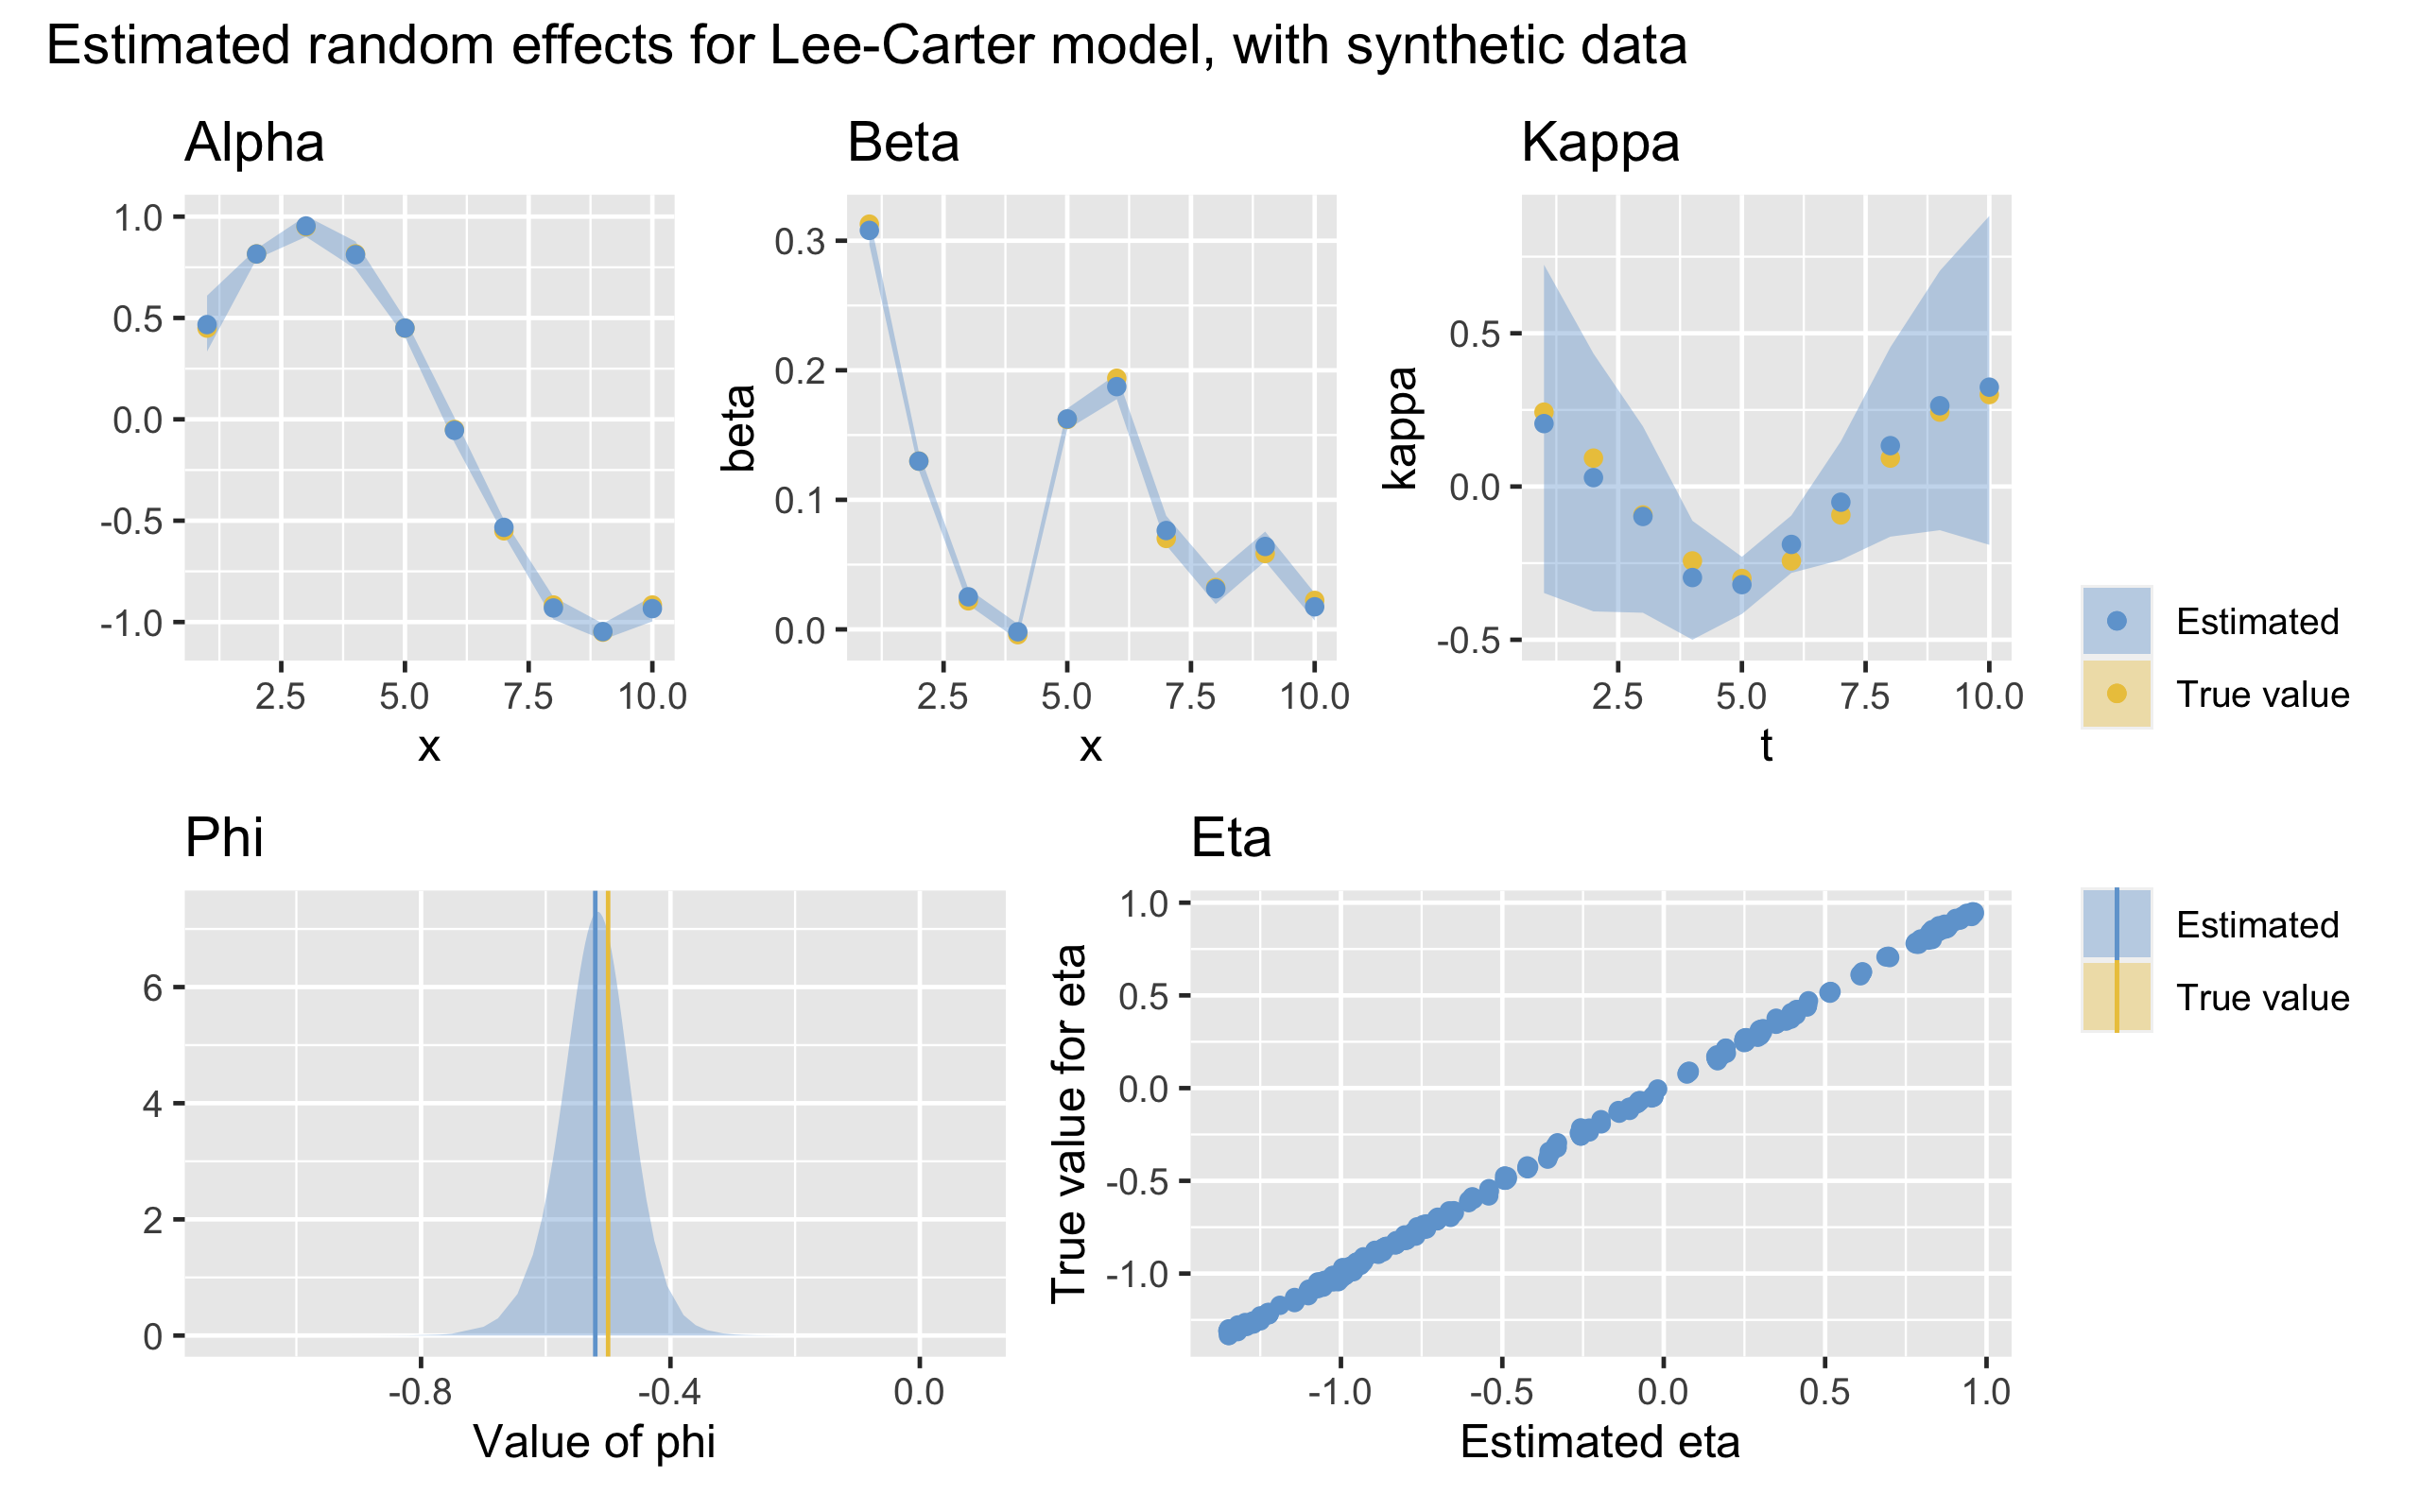
\includegraphics[width=\textwidth]{synthetic-data/Figures/effects-LC-synthetic.png}
        \caption{\textit{Top:} The mean and the 95\% confidence bounds of the approximated posterior marginal distributions of $\alpha_x$ (Alpha), $\beta_x$ (Beta) and $\kappa_t$ (Kappa), together with their respective true random effects. \textit{Bottom, left:} The approximated marginal posterior distribution of $\phi$ with the mean value as a solid line, together with the true value of $\phi$. \textit{Bottom, right:} The mean of the approximated posterior marginal distribution for $\eta_{x,t}$ plotted against the true value for $\eta_{x,t}$. }
        \label{fig:firstRun-top}
    \end{subfigure}
    
    \begin{subfigure}[b]{0.6\textwidth}
        \centering
        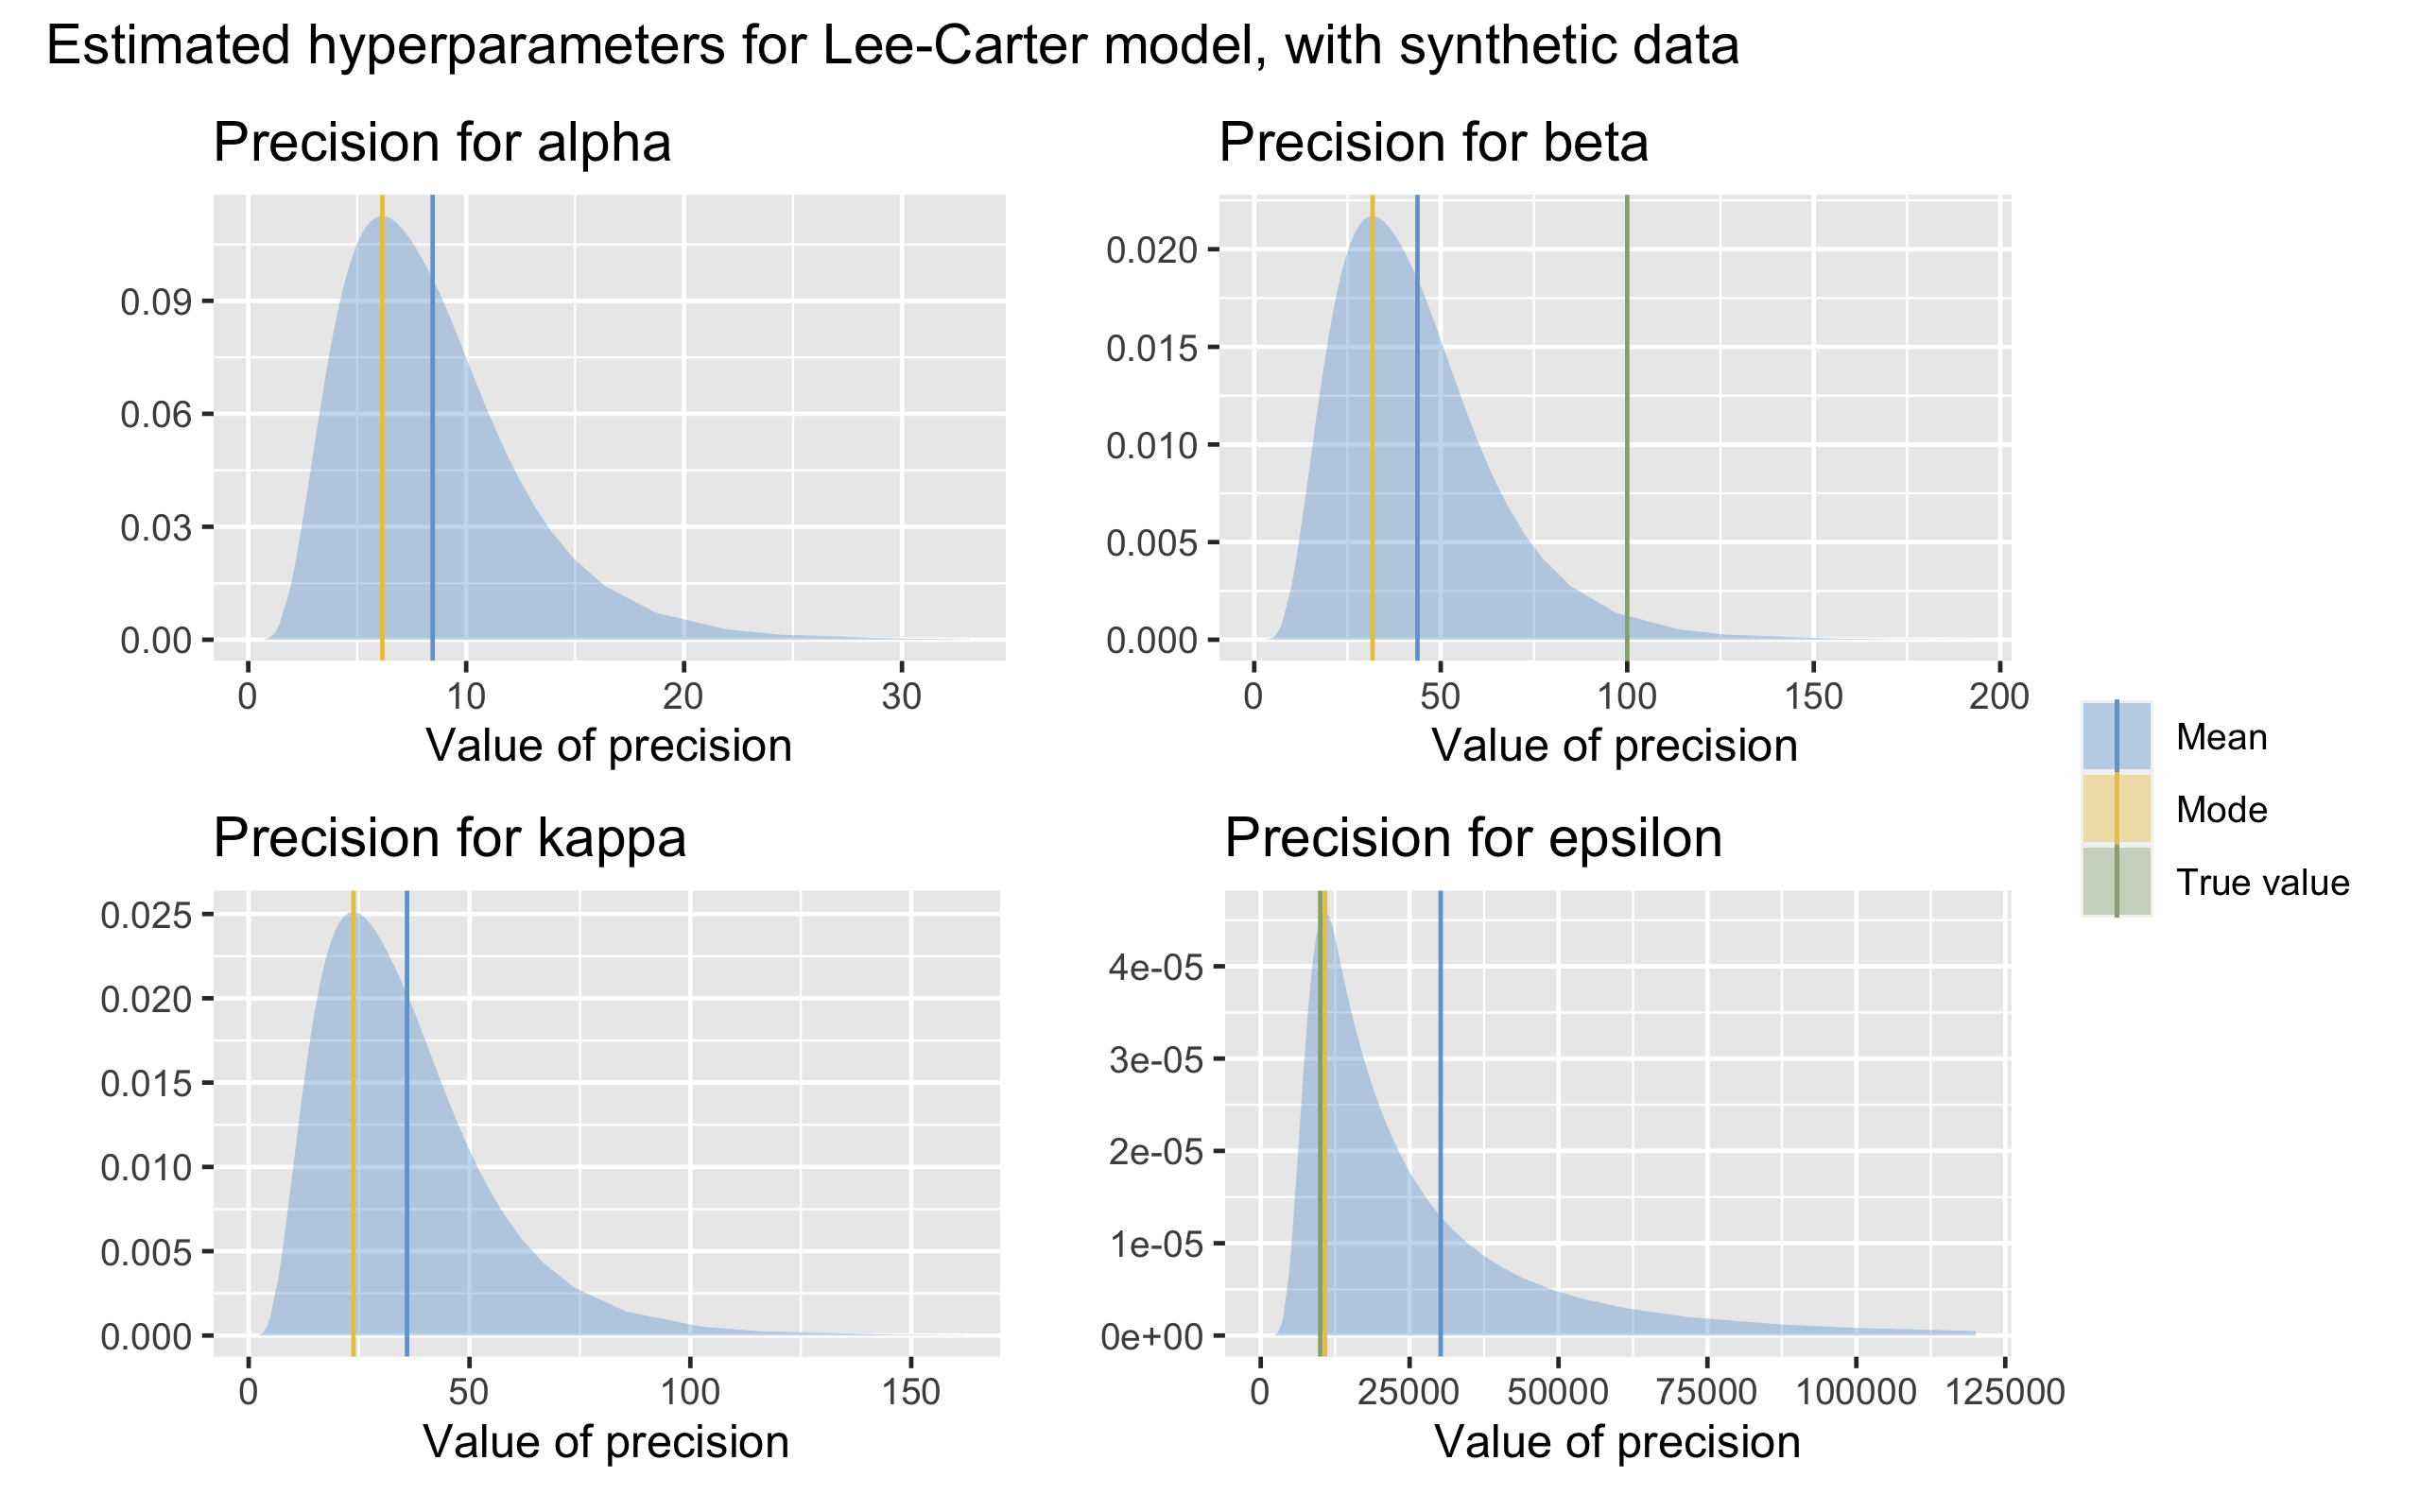
\includegraphics[width=\textwidth]{synthetic-data/Figures/hyperparameters-LC-synthetic-2-1.png}
        \caption{The estimated marginal distributions with their means and modes, for the precisions $\tau_\alpha$, $\tau_\beta$ and $\tau_\kappa$ of the random effects $\alpha_x$, $\beta_x$ and $\kappa_t$, as well as $\tau_\epsilon$ for the random term $\epsilon_{x,t}$. The precisions used to sample underlying values for $\beta_x$ and $\epsilon_{x,t}$ is marked with green lines.}
        \label{fig:firstRun-bottom}
    \end{subfigure}
    
    \caption{The results from running \inlabru when the random effects are simulated from the model given in Expression \ref{eq:conf21}. }
    \label{fig:firstRun}
\end{figure}
\newpar From Figure \ref{fig:firstRun-top} it is clear that \inlabru is able to identify all random effects significantly, as well as displaying a good estimation for the predictor $\eta_{x,t}$ (A straight line with a slope of one in the plot of estimated and true values of $\eta_{x,t}$ correspond to equal values). From Figure \ref{fig:firstRun-bottom}, we see that that the estimated and the real value of $\tau_\beta$ and $\tau_\epsilon$ are of the same order of magnitude, which indicates a good fit, even though we should note that the estimated value of $\tau_\beta$ is lower than the true value of $\tau_\beta$. Since we do not sample the values of $\alpha_x$ and $\kappa_t$ using $\tau_\alpha$ or $\tau_\kappa$ explicitly, we do not conclude on the correctness of these values. 

\newpar We perform this procedure for several other combinations of functions for the random effects as well. We observe that \inlabru is able to produce a good result for the predictor $\eta_{x,t}$ in all cases and good results for the random effects in most cases. In Section \ref{sec:IdentifiabilityKappa} we discuss why the combination of random effects that yield bad results from \inlabru are not considered realistic, and then not a hinder for using \inlabru to fit LC-models. These results provide the basis for for our paper, as it shows that \inlabru makes it possible to bypass the obstacle that \inla alone is not able to handle Lee-Carter type models with non-linear predictors.

% old version:

% \noindent To produce the synthetic data, we choose functions for $\alpha_x$, $\beta_x$ and $\kappa_t$ and a $\phi$ that we believe to be somewhat realistic: $\alpha_x$ is modeled both as a constant (i.e. included in the intercept $\mu$) and as different functions and realizations of random walks, $\kappa_t$ are modeled as different functions and realizations of random walks and $\beta_x$ is modeled as 
% \begin{equation*}
%     \beta_x \sim \Normal(0,1/\tau)
% \end{equation*} 
% for some precisions $\tau$. We sample the random terms $\epsilon_{x,t}$ from an iid normal distribution with zero mean and precision $\tau_\epsilon$. $\alpha_x$, $\beta_x$ and $\kappa_t$ are then scaled to their respective constraints, given in \ref{eq:LCconstraintsFinal}. As we expect \inlabru to handle any sufficiently smooth and close-to-realistic effects to accept it as a suitable inference tool for the LC and LCC model, we do not attach a lot of importance to the choices for the synthetic models for the random effects. 
% The \inlabru method was run for multiple configurations of the true effects. Figure \ref{fig:firstRun} displays the results from the run when the random effects were modelled as
% \begin{equation}
%     \begin{aligned}
%     \alpha_x &= \cos(\frac{x-3}{6}\pi)\\
%     \beta_x &= \Normal(0,0.1^2)\\
%     \phi &= -0.5\\
%     \kappa_t &= 0.3\cos(\frac{t\cdot \pi}{5})\\
%     \tau_{\epsilon} &= 1/0.01^2.
%     \end{aligned}
%     \label{eq:conf21}
% \end{equation}
% for $x\in [1,10]$ and $t \in [1,10]$. The code used to produce these results can be found at the \texttt{GitHub} repository under \texttt{synthetic-data/L-C-alpha-x.R}. 


% From Figure \ref{fig:firstRun-top} it is clear that \inlabru is able to identify all random effects significantly, as well as displaying a good estimation for the predictor $\eta_{x,t}$ (A straight line with a slope of one in the plot of estimated and true values of $\eta_{x,t}$ correspond to equal values). Looking at the results from testing \inlabru with other models for the random effects, we observe that \inlabru is able to produce a good result for the predictor $\eta_{x,t}$ in all cases and good results for the random effects in most cases. In Section \ref{sec:IdentifiabilityKappa} we discuss why the combination of random effects that yield bad results from \inlabru are not considered realistic, and then not a hinder for using \inlabru to fit LC-models. These results provide the basis for for our paper, as it shows that \inlabru makes it possible to bypass the obstacle that \inla alone is not able to handle Lee-Carter type handle models with non-linear predictors.

\subsection{Implementation of $\beta_x$}
In the implementation of the LC-model (\ref{eq:LC-rewritten}) in \texttt{R}, the multiplicative term of the predictor $\etax$ is entered as
\begin{equation}
    \beta_x\cdot\phi \cdot t + \beta_x\kappa_t,
\end{equation}
so that the $\beta_x$ effect exists in two terms. There are two ways to handle this when using the \texttt{R} \inlabru library. The first option, which is specific to the \inlabru method, is to use the same component for $\beta_x$ in both terms. This is implemented (for the simplest LC-model where $\alpha_x$ is included in the intercept) in the \texttt{components} object and the \texttt{formula} object as:
\begin{verbatim}
comp.single = ~ Intercept + 
    phi(t, model = "linear") + 
    beta(x, model = "iid", extraconstr = list(A = A.mat, e = e.vec)) + 
    kappa(t1, model = "rw1", values = 1:nt, constr = TRUE, hyper = pc.prior) + 
    epsilon(xt, model = "iid")
form.single = y ~ Intercept + beta*phi + beta*kappa + epsilon
\end{verbatim}
In Section \ref{sec:synthFirstInferenceLC} this implementation was used. The second option, is to define two different components for $\beta_x$, and to use the \texttt{copy}-feature in \inla to make one component a copy of the other, plus some small noise \parencite{MARTINS201368}. This implementation is the one that is used for similar models in the plain \inla method. It is implemented as
\begin{verbatim}
comp.copy = ~ Intercept + 
    phi(t, model = "linear") + 
    beta1(x, model = "iid", extraconstr = list(A = A.mat, e = e.vec)) + 
    kappa(t1, model = "rw1", values = 1:nt, constr = TRUE, hyper = pc.prior) + 
    beta2(x1, model = "iid", copy="beta1") +
    epsilon(xt, model = "iid")
form.copy = y ~ Intercept + beta1*phi + beta2*kappa + epsilon
\end{verbatim}
We investigate whether both approaches can be used to fit our model, and if so, which one performs the best. The code used to produce these results can be found at the \texttt{GitHub} repository under \texttt{synthetic-data/L-C-copy-beta.R}. 

\begin{figure}[h!]
    \centering
    \begin{subfigure}[b]{0.85\textwidth}
        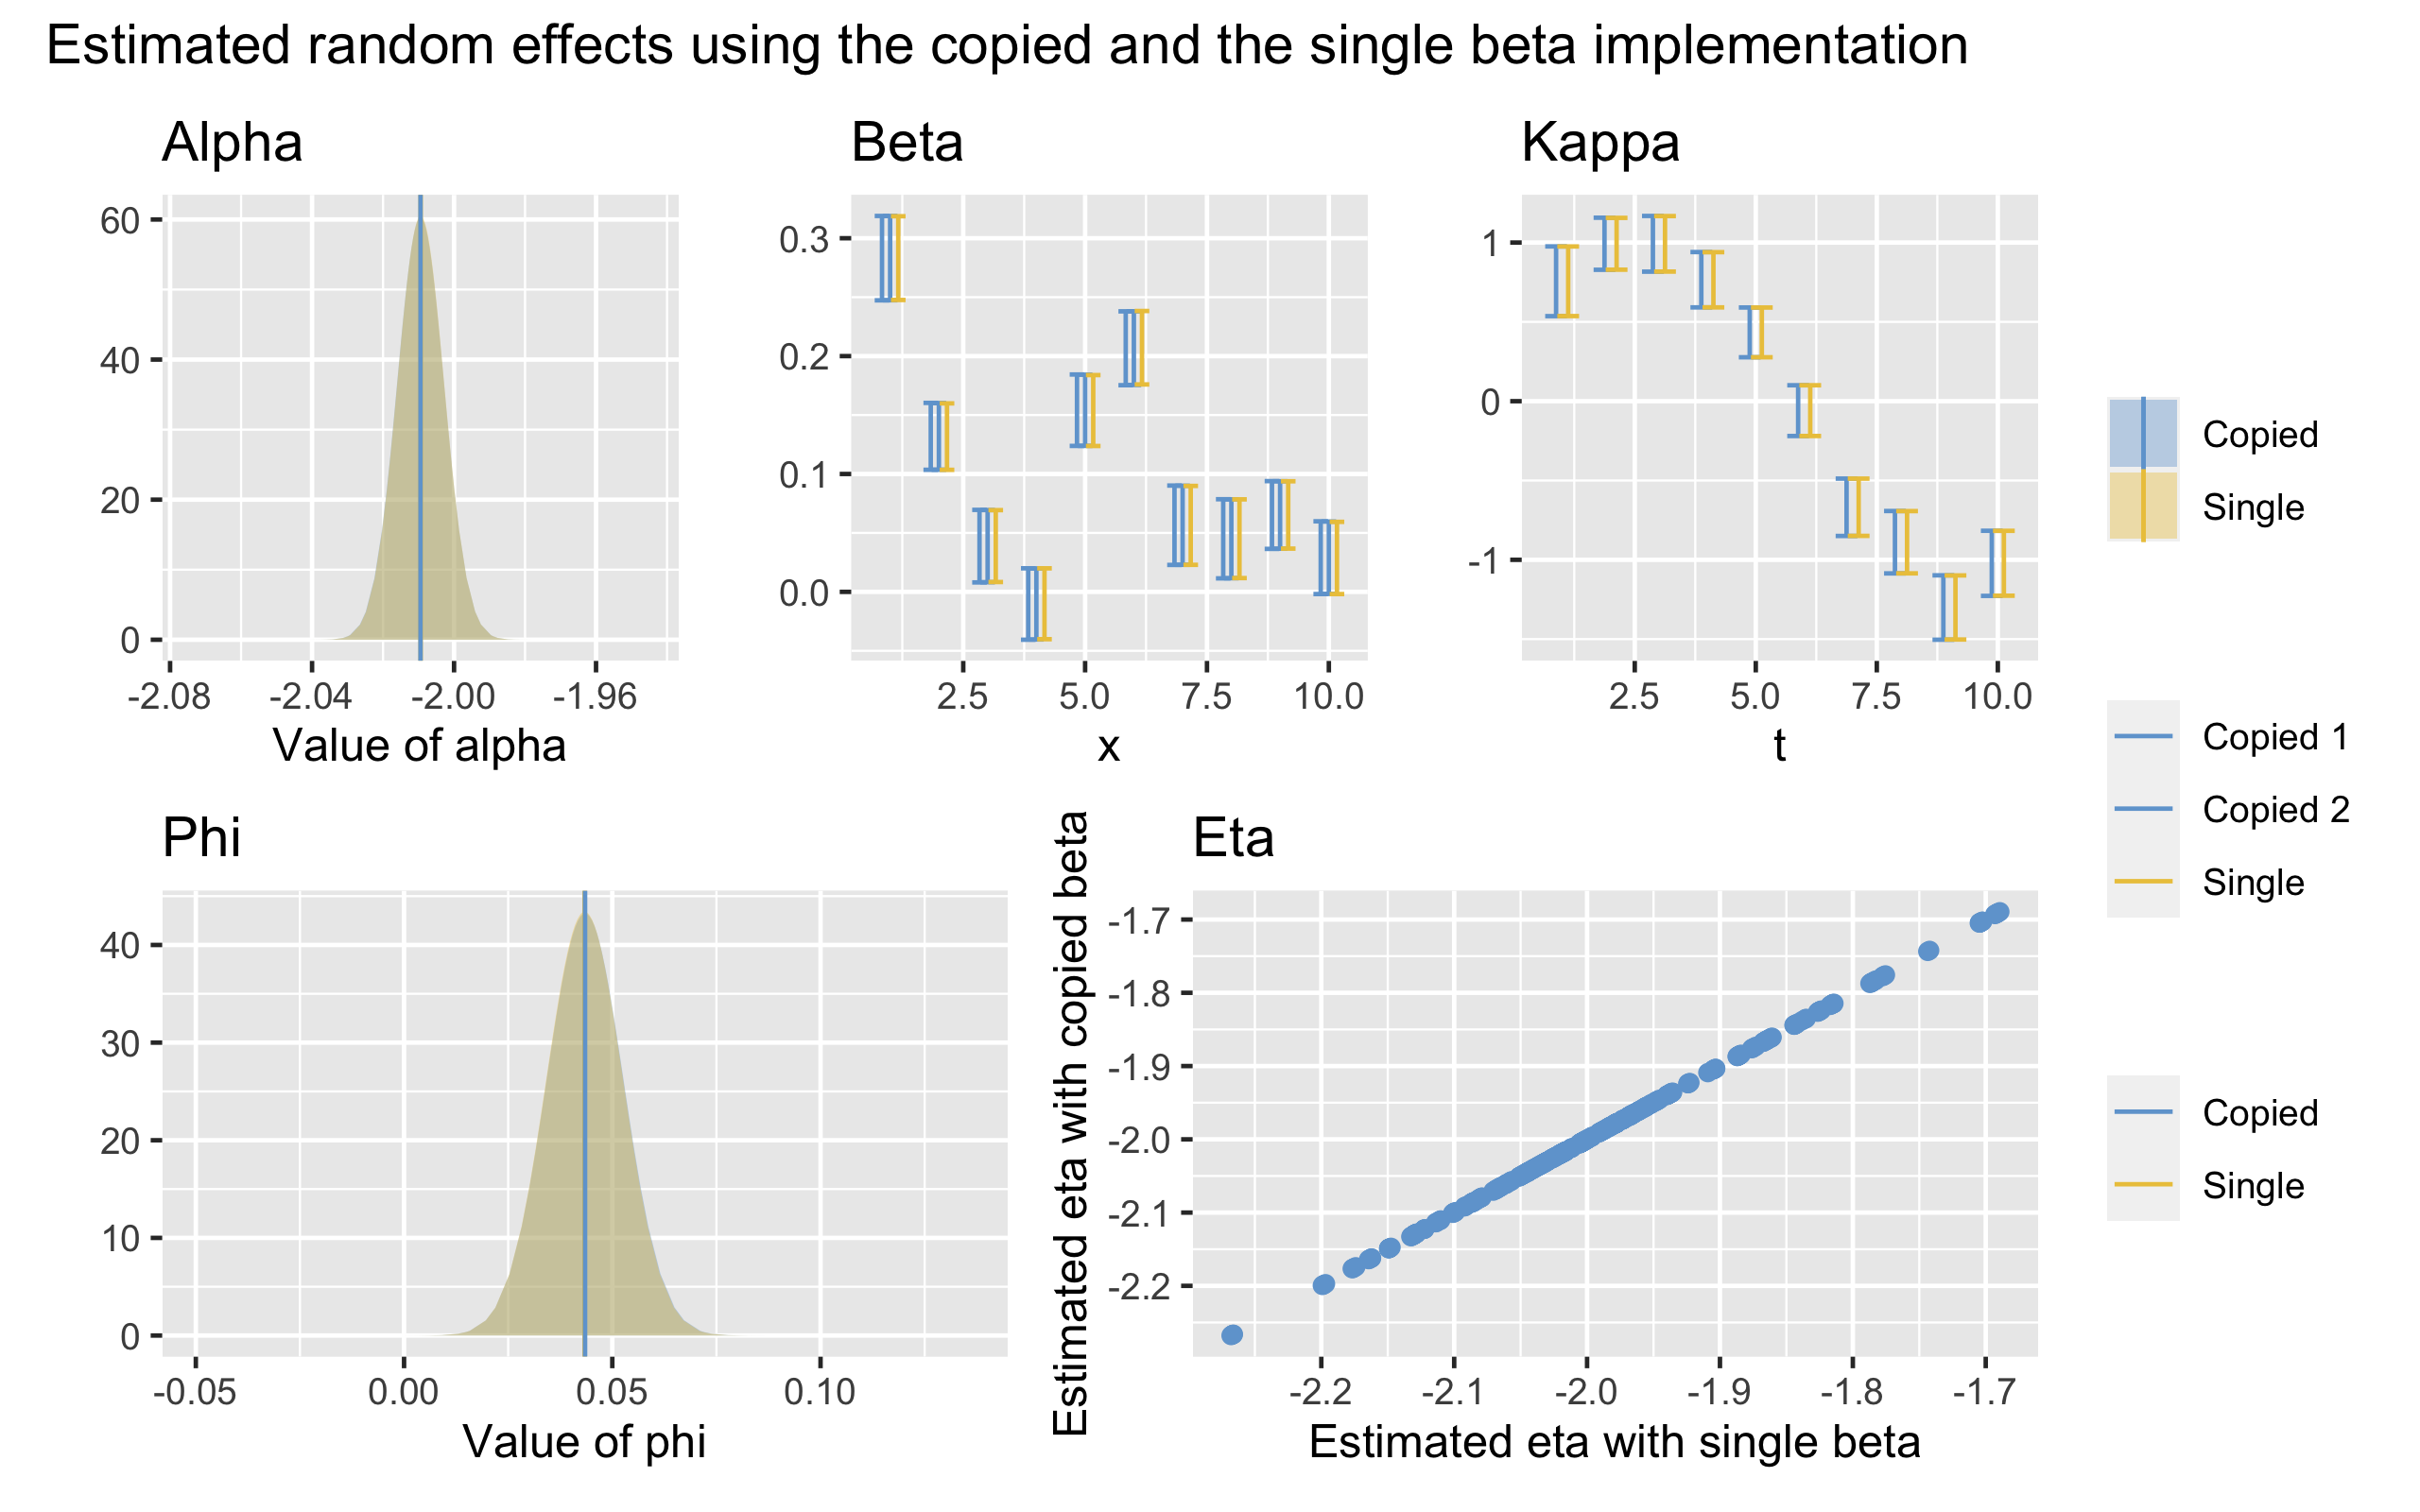
\includegraphics[width=\textwidth]{synthetic-data/Figures/copy-beta.png}
        \caption{\textit{Top:} The posterior marginal distributions for $\alpha_x$, and the 95\% confidence bounds for the marginal posteriors of $\beta_x$ and $\kappa_t$, with and without the \texttt{copy} feature. \textit{Bottom, left:} The approximated marginal posterior distribution of $\phi$ with the mean value as a solid line, with and without the \texttt{copy} feature. \textit{Bottom, right:} The mean of the approximated posterior marginal distribution for $\eta_{x,t}$ from the implementation with the \texttt{copy} feature plotted against the value for $\eta_{x,t}$ from the implementation without the \texttt{copy} feature. }
        \label{fig:copyBetaComparison-top}
    \end{subfigure}
    
    \begin{subfigure}[b]{0.6\textwidth}
        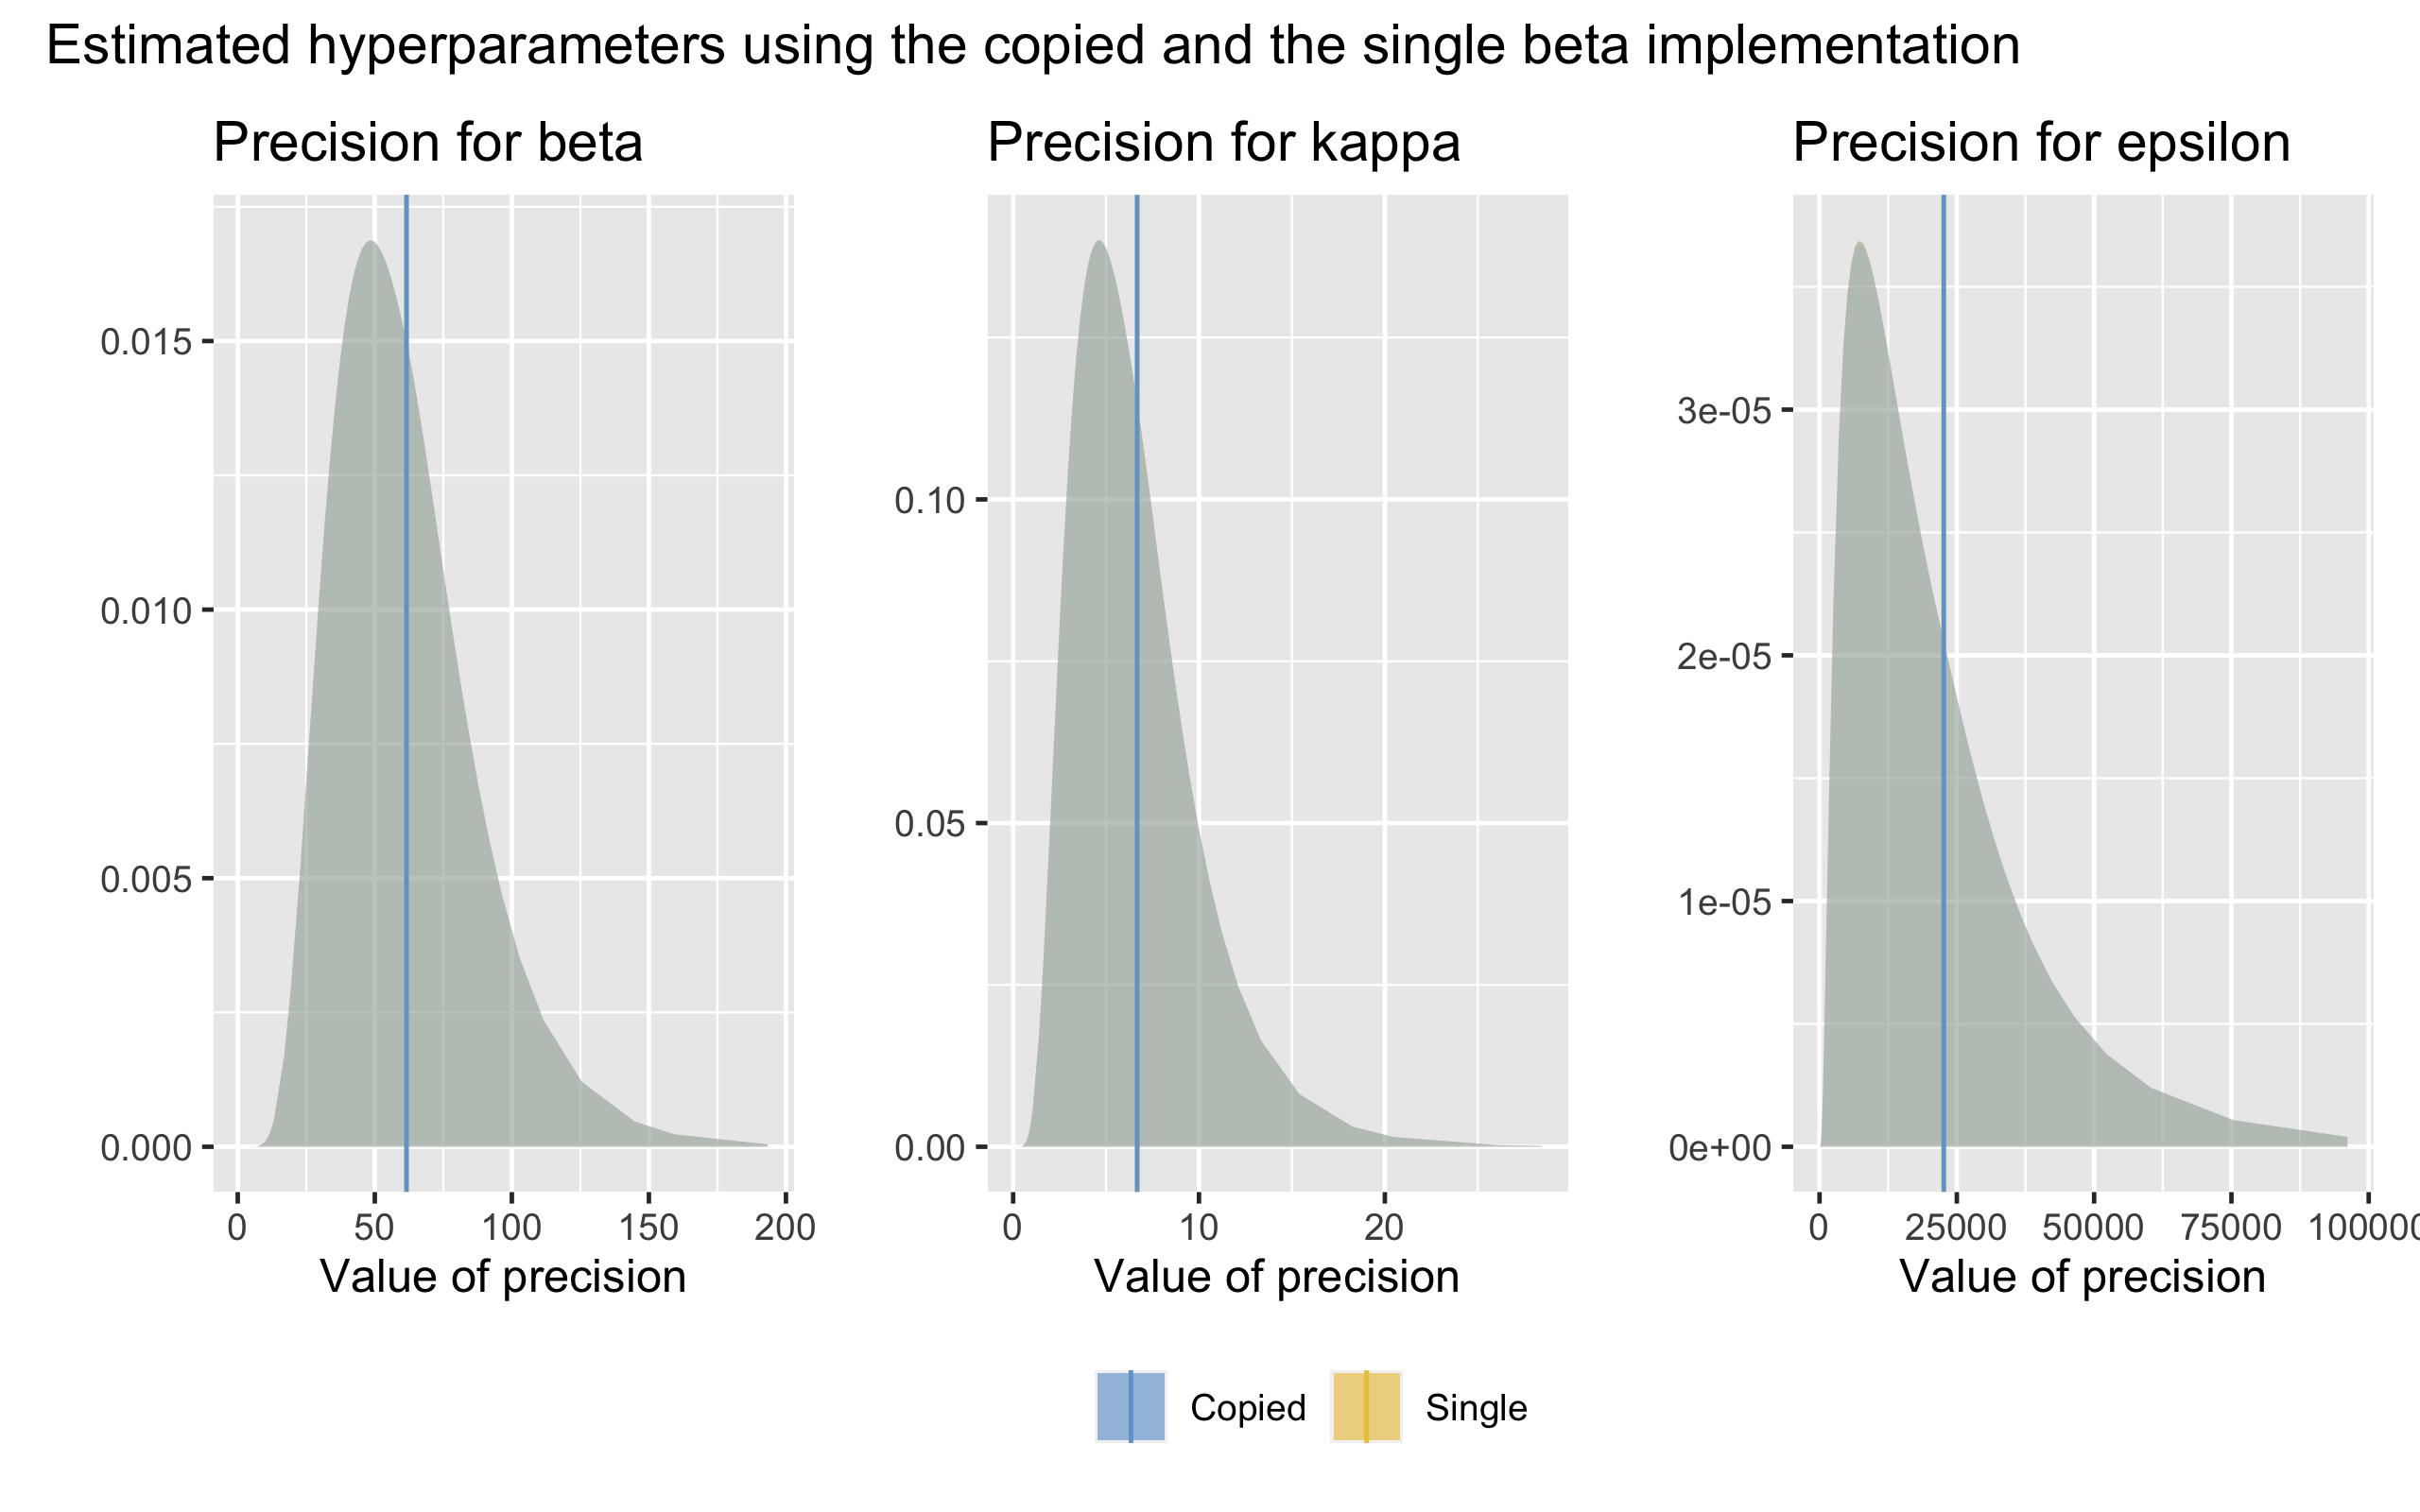
\includegraphics[width=\textwidth]{synthetic-data/Figures/hyperparameters-LC-copy.png}
        \caption{The estimated hyperparameters, $\tau_\beta$, $\tau_\kappa$ and $\tau_\epsilon$ when using the $\texttt{copy}$-feature and when not using the $\texttt{copy}$-feature}
        \label{fig:copyBetaComparison-bottom}
    \end{subfigure}
    \caption{Comparison of estimation results from running \inlabru on the same underlying model with two versions of the implementation, with and without the $\texttt{copy}$-feature.}
    \label{fig:copyBetaComparison}
\end{figure}

\begin{figure}[h!]
    \centering
    \begin{subfigure}[b]{0.45\textwidth}
        \centering
        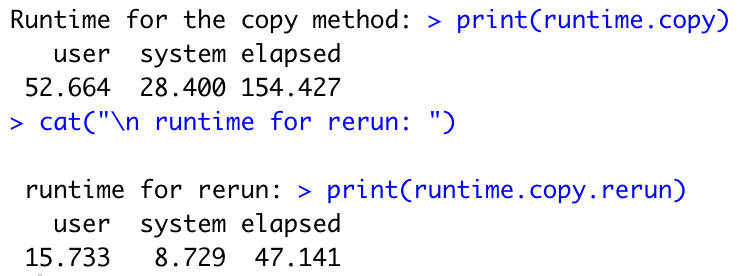
\includegraphics[trim=0 5 0 0,clip,width=\textwidth]{synthetic-data/Figures/runtime-copy.png}
    \end{subfigure}
    \begin{subfigure}[b]{0.45\textwidth}
        \centering
        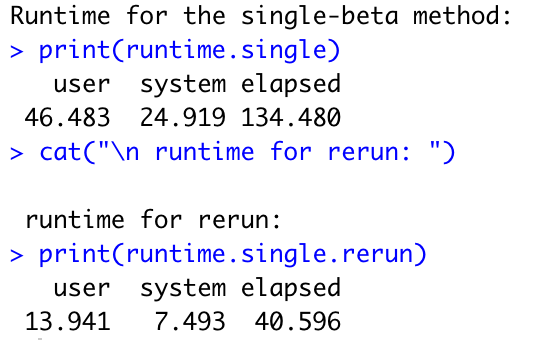
\includegraphics[trim=0 0 15 0,clip, width=\textwidth]{synthetic-data/Figures/runtime-single.png}
    \end{subfigure}
    \caption{The run time of running \inlabru inference using the $\texttt{copy}$-feature (right) and without using the $\texttt{copy}$-feature (left).}
    \label{fig:copyBetaRuntimes}
\end{figure}

\newpar A comparison between the results from the two runs with the different implementations is displayed in Figure \ref{fig:copyBetaComparison} and the corresponding run times are shown in Figure \ref{fig:copyBetaRuntimes}. We do not observe any difference in the accuracy of the results from the two implementations, they seem to produce exactly the same results. From Figure \ref{fig:copyBetaRuntimes} we observe that the implementation using the $\texttt{copy}$-feature seemed to take slightly more time to run. Even through this difference in run time is not necessarily significant, we still do not want to unnecessarily complicate our implementations, and we do not use the \texttt{copy}-feature in the remaining simulations.

\subsection{Identifiability Issues with $\kappa_t$ and $\phi\cdot t$}
\label{sec:IdentifiabilityKappa}
For some combinations of underlying models for $\kappa_t$ and $\phi$ we observe that \inlabru is not able to correctly identify these effects, while the predictions of $\eta_{x,t}$ are still correct, as mentioned in Section \ref{sec:synthFirstInferenceLC}. This indicates that there are some identifiability issues between $\kappa_t$ and $\phi \cdot t$ that become apparent for some combinations of these effects. We test several different combinations of $\kappa_t$ and $\phi$ to try to isolate the types of combinations that \inlabru is not able to correctly identify.
\begin{figure}[h!]
    \centering
    \begin{subfigure}[b]{0.85\textwidth}
        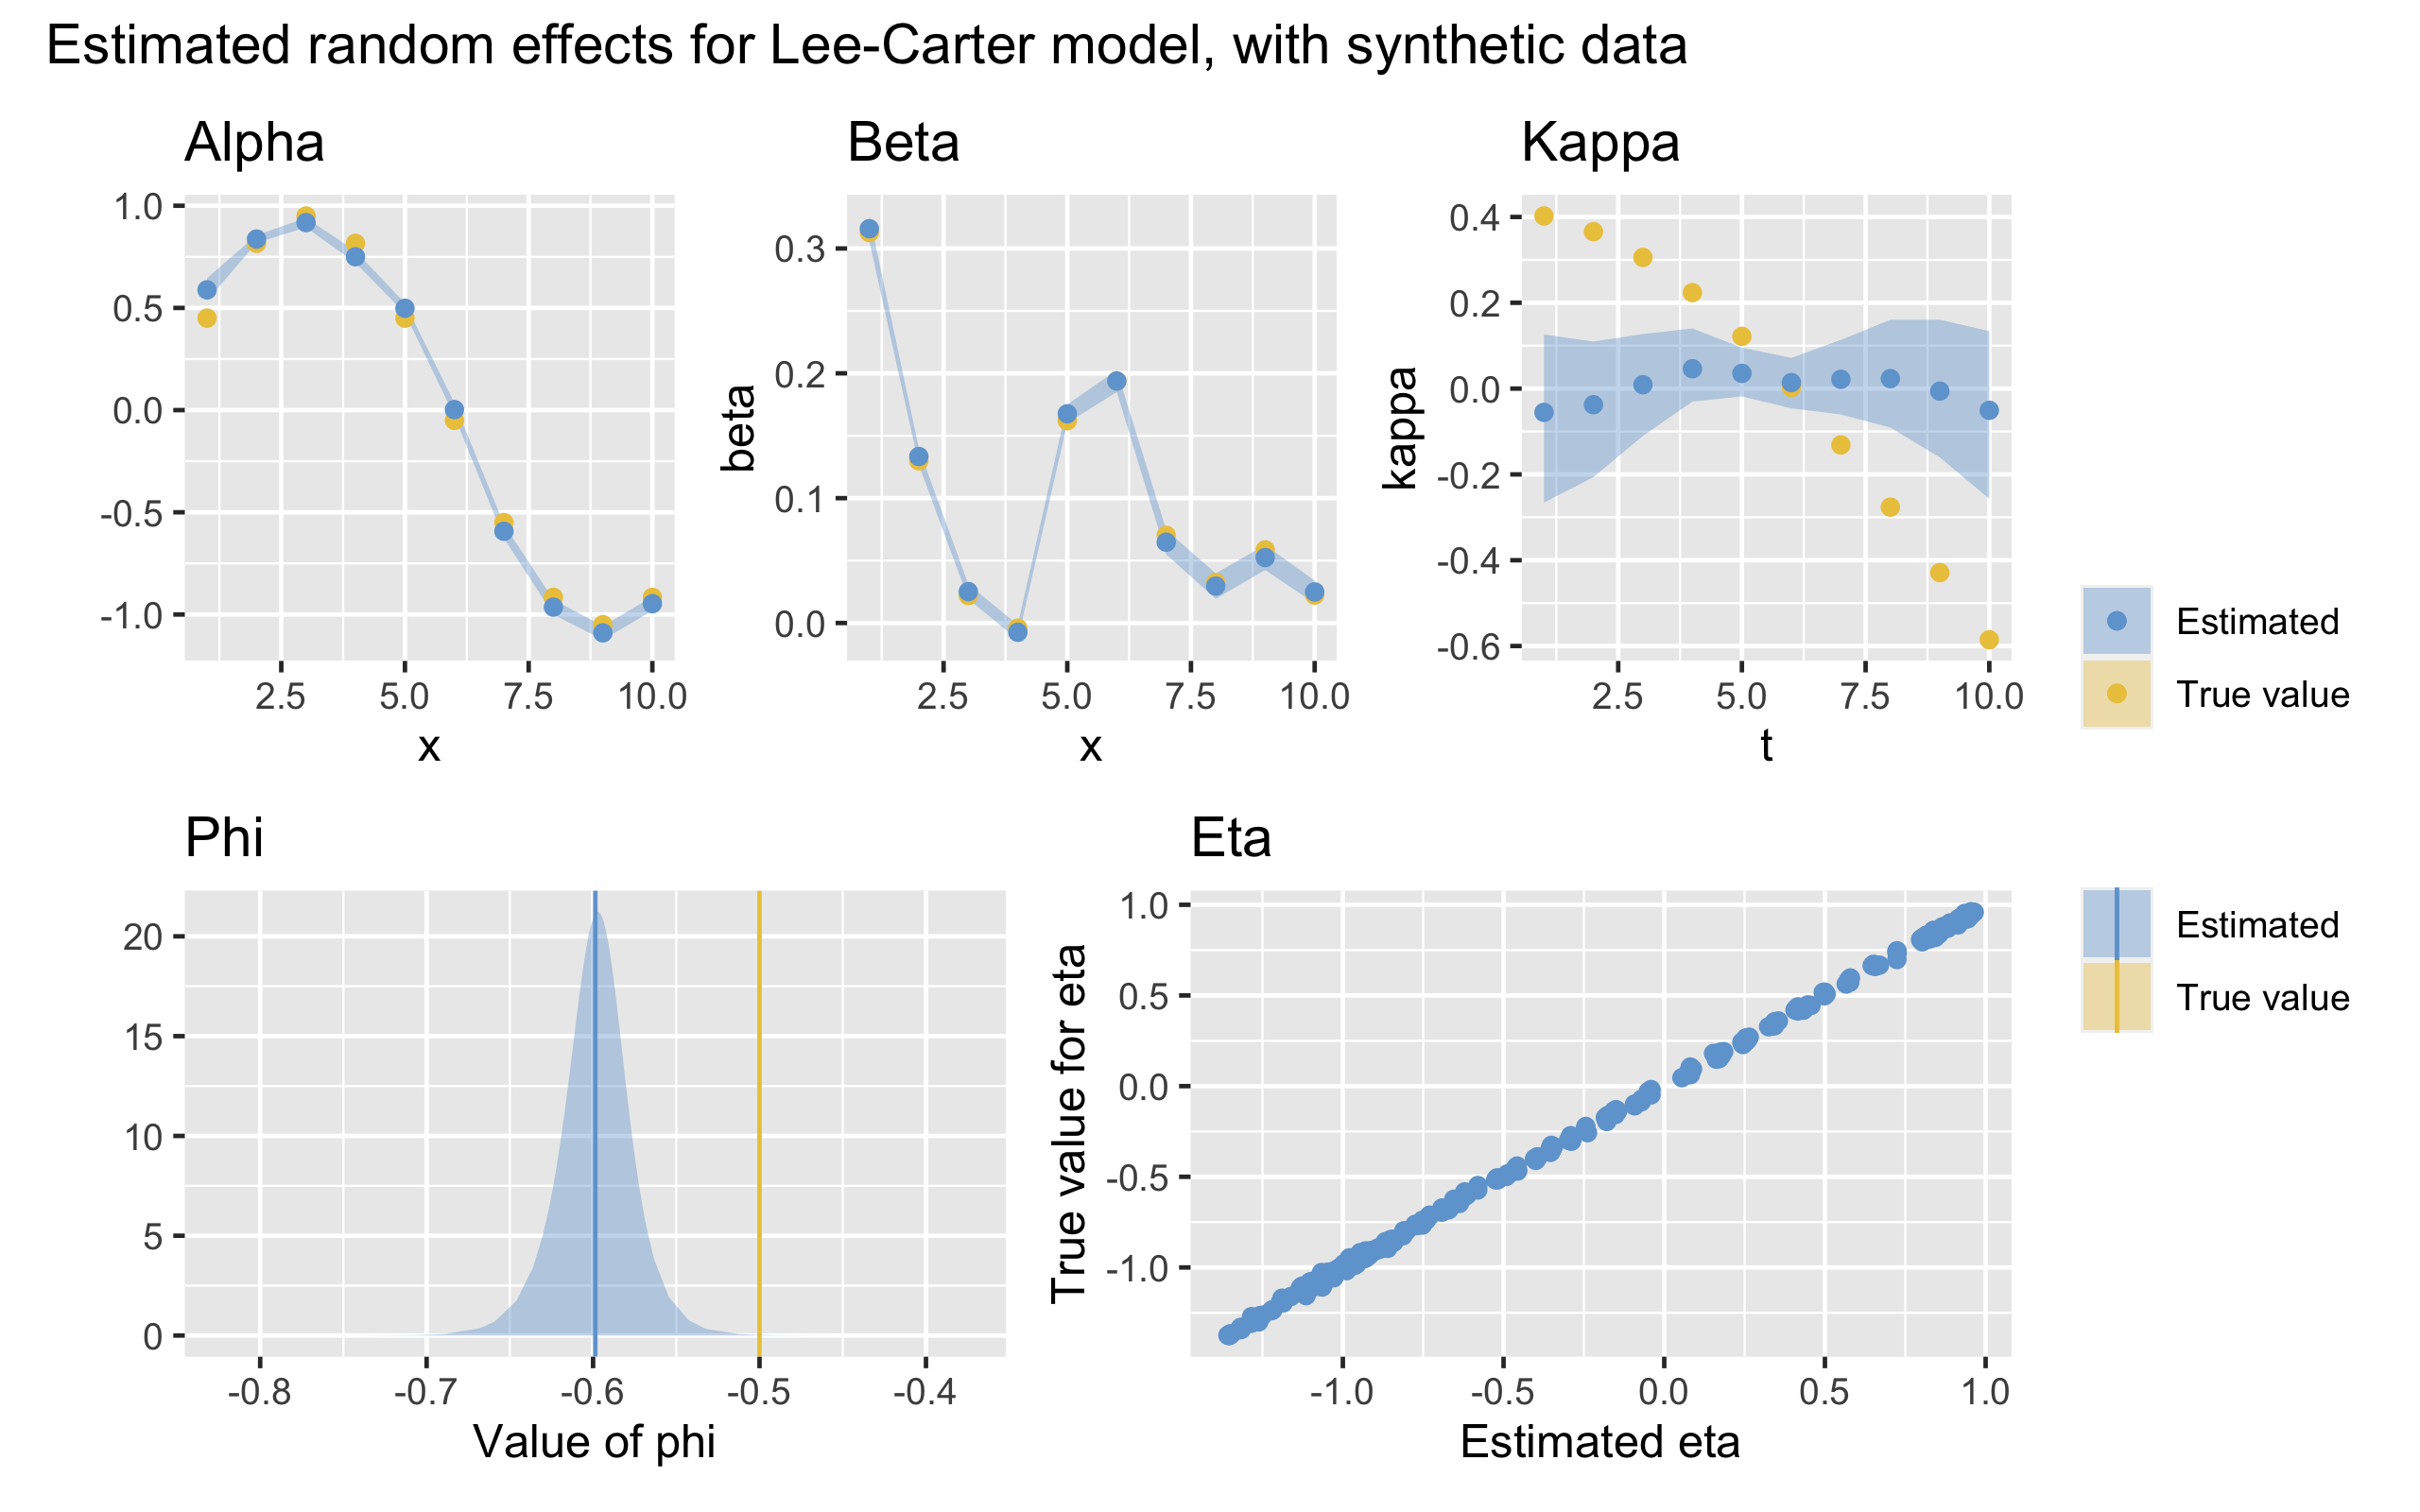
\includegraphics[width=\textwidth]{synthetic-data/Figures/effects-LC-synthetic-identifiability.png}
        \caption{The estimated random effects $\alpha_x$, $\beta_x$, $\phi$ and $\kappa_t$, and the estimated predictor $\eta_{x,t}$}
        \label{fig:unidentifiabilityKappa-top}
    \end{subfigure}
    
    \begin{subfigure}[b]{0.6\textwidth}
        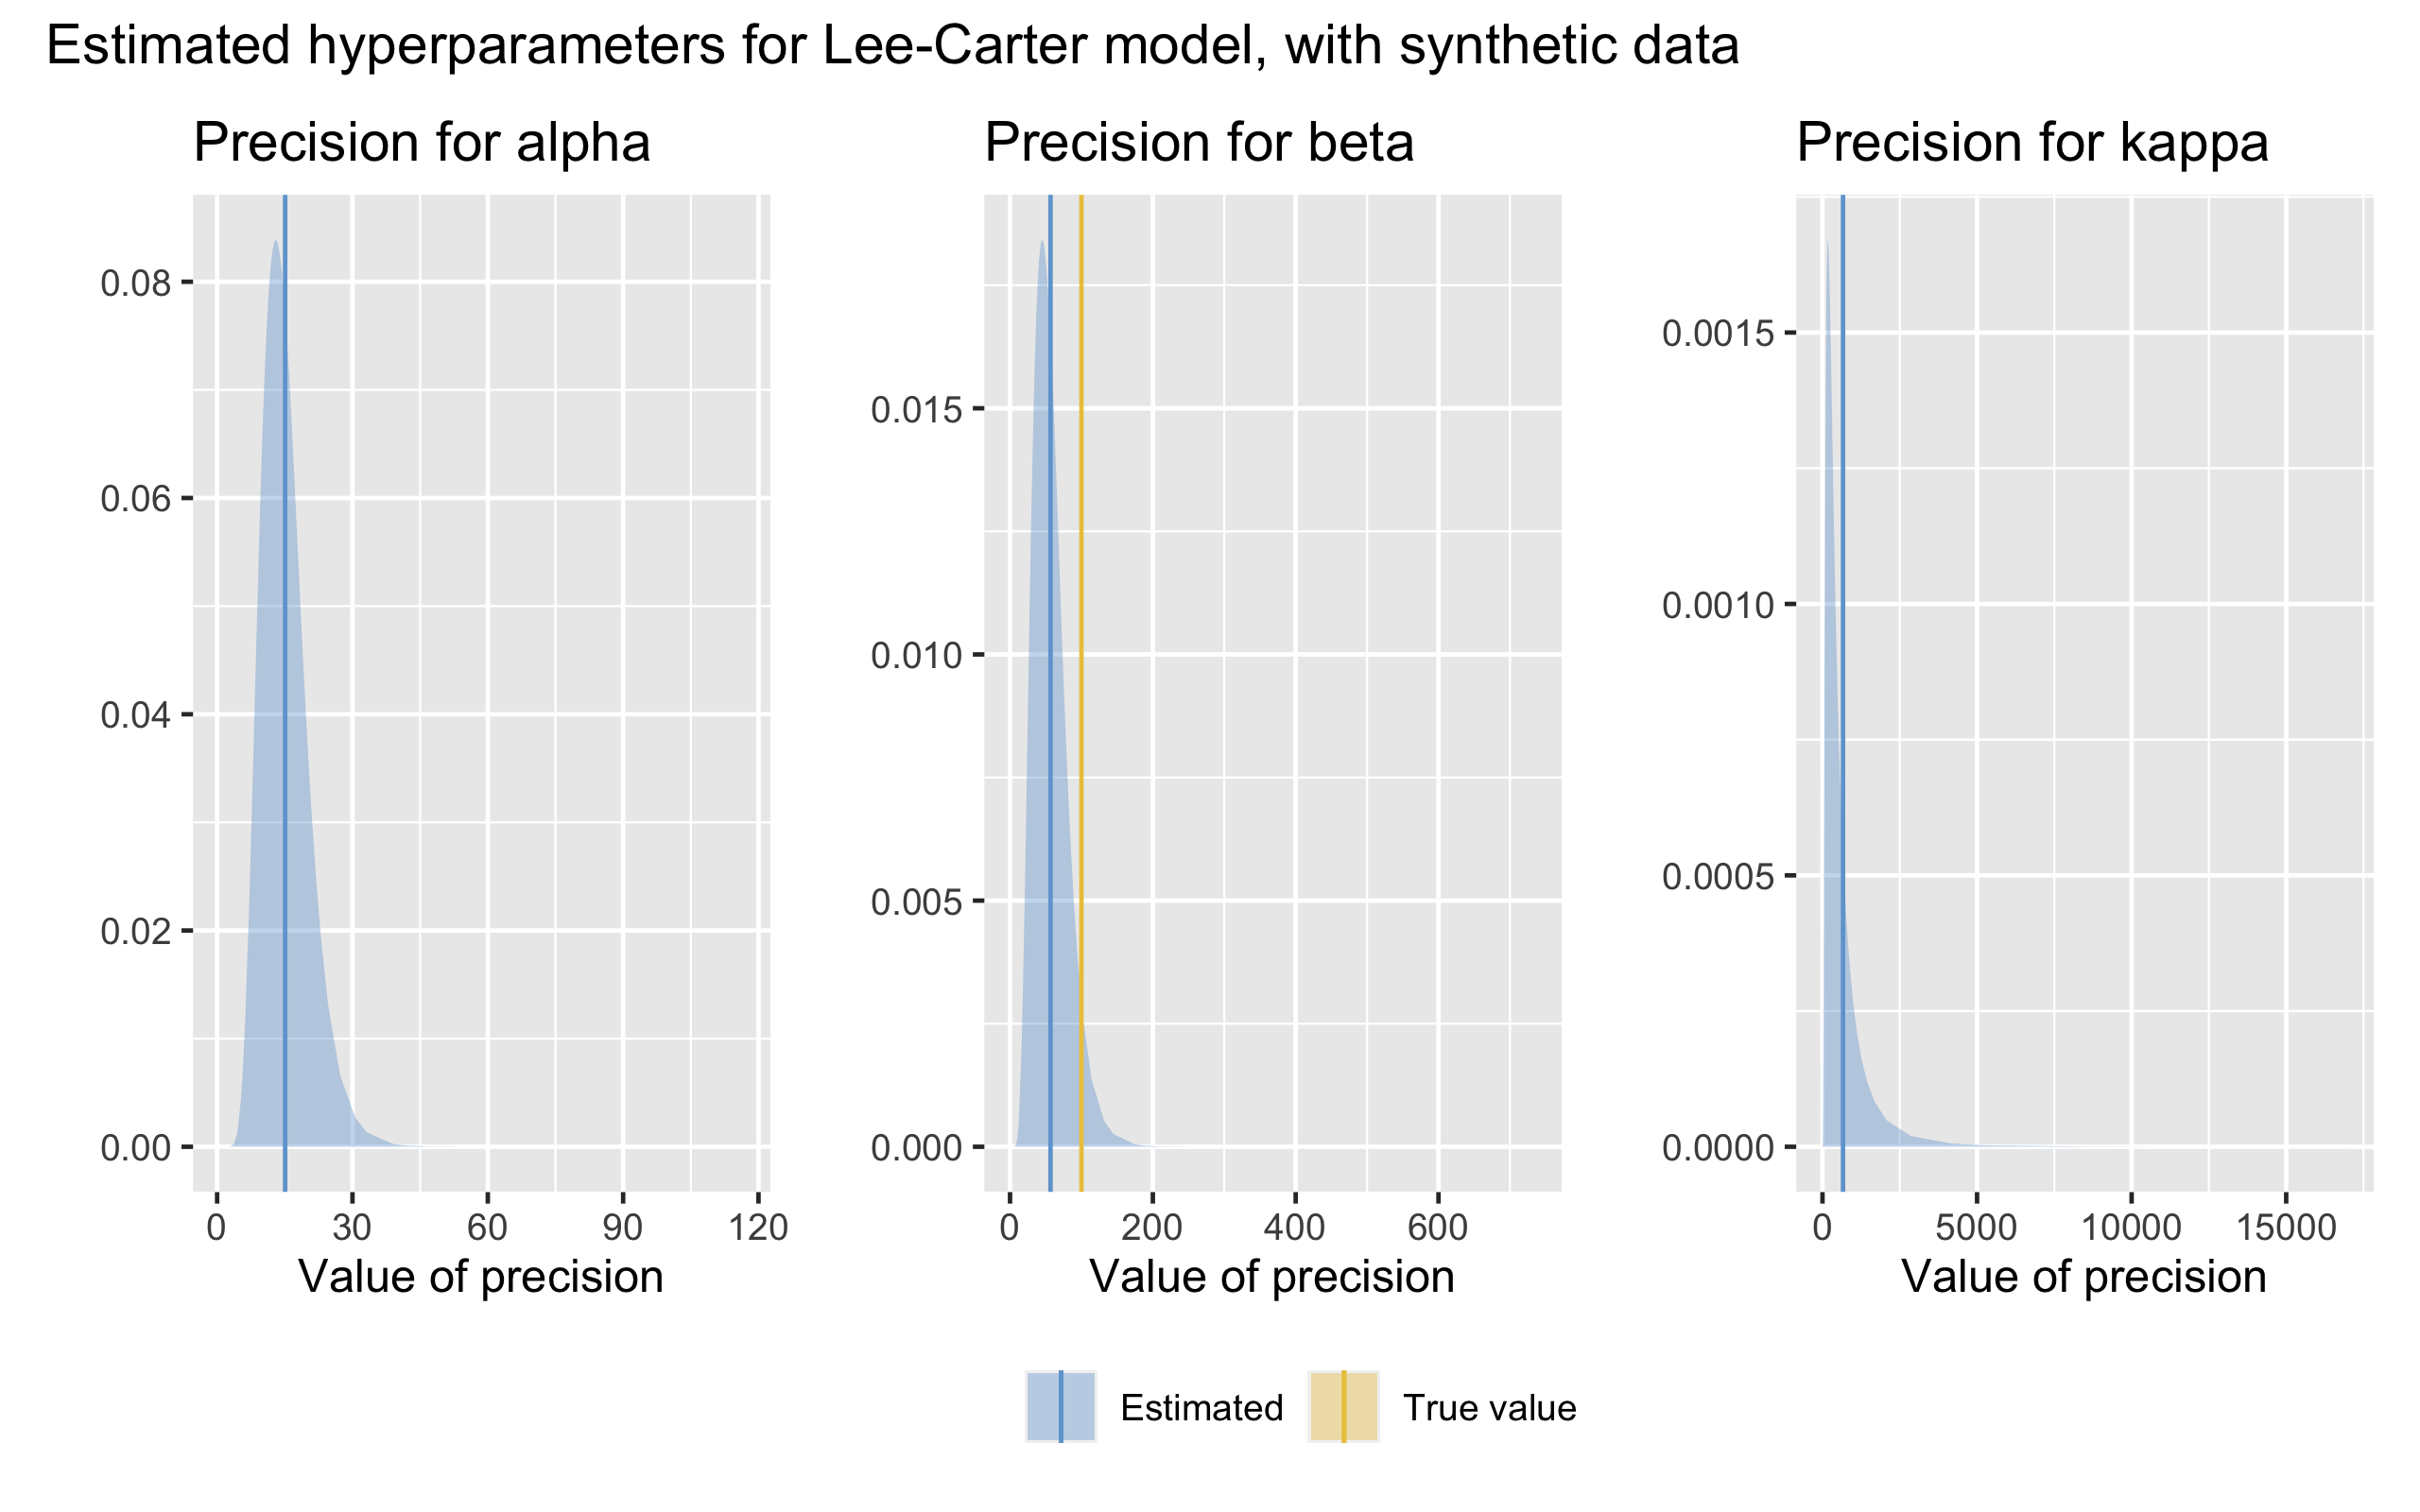
\includegraphics[width=\textwidth]{synthetic-data/Figures/hyperparameters-LC-synthetic-2-2.png}
        \caption{The estimated precisions $\tau_\alpha$, $\tau_\beta$ and $\tau_\kappa$ and $\tau_\epsilon$.}
        \label{fig:unidentifiabilityKappa-bottom}
    \end{subfigure}
    
    \caption{An example of the results after running \inlabru with a configuration that yields identifiability issues with $\kappat$ and $\phi \cdot t$. The plot layout is similar to that of Figure \ref{fig:firstRun}.}
    \label{fig:unidentifiabilityKappa}
\end{figure}
Figure \ref{fig:unidentifiabilityKappa} displays the results from running \inlabru on the following configuration of random effects:
\begin{equation}
    \begin{aligned}
    \alpha_x &= \cos(\frac{x-3}{6}\pi)\\
    \beta_x &= \Normal(0,0.1^2)\\
    \phi &= -0.5\\
    \kappa_t &= \cos(\frac{t\cdot \pi}{20})\\
    \tau_{\epsilon} &= 1/0.01^2.
    \end{aligned}
\end{equation}
for $x\in[1,10]$ and $t\in[1,10]$, where $\alpha_x$, $\beta_x$ and $\kappa_t$ are adjusted to the constraints in Expression \ref{eq:LCconstraintsFinal}. The code used to produce these results can be found at the \texttt{GitHub} repository under \texttt{synthetic-data/L-C-alpha-x.R}. From Figure \ref{fig:unidentifiabilityKappa-top} we clearly see errors in the approximations of $\kappa_t$ and $\phi\cdot t$ while the approximations of $\eta_{x,t}$ (and $\beta_x$ and $\alpha_x$) are close to the true values. From Figure \ref{fig:unidentifiabilityKappa-bottom} we observe that the marginal distribution of the precision $\tau_\kappa$ is very wide, indicating a high uncertainty in the estimated value for this hyperparameter. We observe, from these and other similar results, that \inlabru produces incorrect estimations for $\kappa_t$ and $\phi$ when the underlying model for $\kappa_t$ show too clear drift tendencies. This indicates that \inlabru places all drift along the period axis in the linear term $\phi$. We can accept this "misplacement", since we have explicitly defined our model as the sum of a random walk without drift and and some linear effect. Even though the realization of a drift-less random walk could easily display drift-like tendencies, we accept the apparent assumption of \inlabru that all drift along the $t$ axis originates from the linear effect $\phi \cdot t$, since we still get good results for the predictor $\eta_{x,t}$, the remaining random effects and the estimated precisions $\tau_\beta$ and $\tau_\epsilon$.
\newline
\subsection{Inference with \inlabru on the LCC-model. }
The next step in our preliminary analysis is to test the performance of \inlabru on the LCC-model. We recall that the LCC-model is given by
\begin{equation}
    Y_{x,t} \sim \Poisson(E_{x,t}\cdot e^{\eta_{x,t}}), \quad \eta_{x,t} = \mu + \alpha_x + \beta_x(\phi \cdot t + \kappa_t) + \gamma_k + \epsilon_{x,t},
    \label{eq:LCC-rewritten-rep1}
\end{equation}
where $x = 1,\ldots,X$, $t = 1,\ldots,T$, $k = 1,\ldots,K$, $Y_{x,t}$ is the number of observed cases (deaths) and $E_{x,t}$ is the at-risk population. The cohort effect is included in the \texttt{R} script in the same manner as the other effects. We simulate the random effects for three different configurations, and we investigate the prediction results. All code used in this phase can be found at \url{https://github.com/Helenerb/Project-thesis/synthetic-data} in the scripts \texttt{L-C-cohort-v2-3-1.R}, \texttt{L-C-cohort-rw.R} and \texttt{L-C-cohort-v2.R}.
\begin{figure}[h!]
    \centering
    \begin{subfigure}[b]{0.85\textwidth}
        \centering
        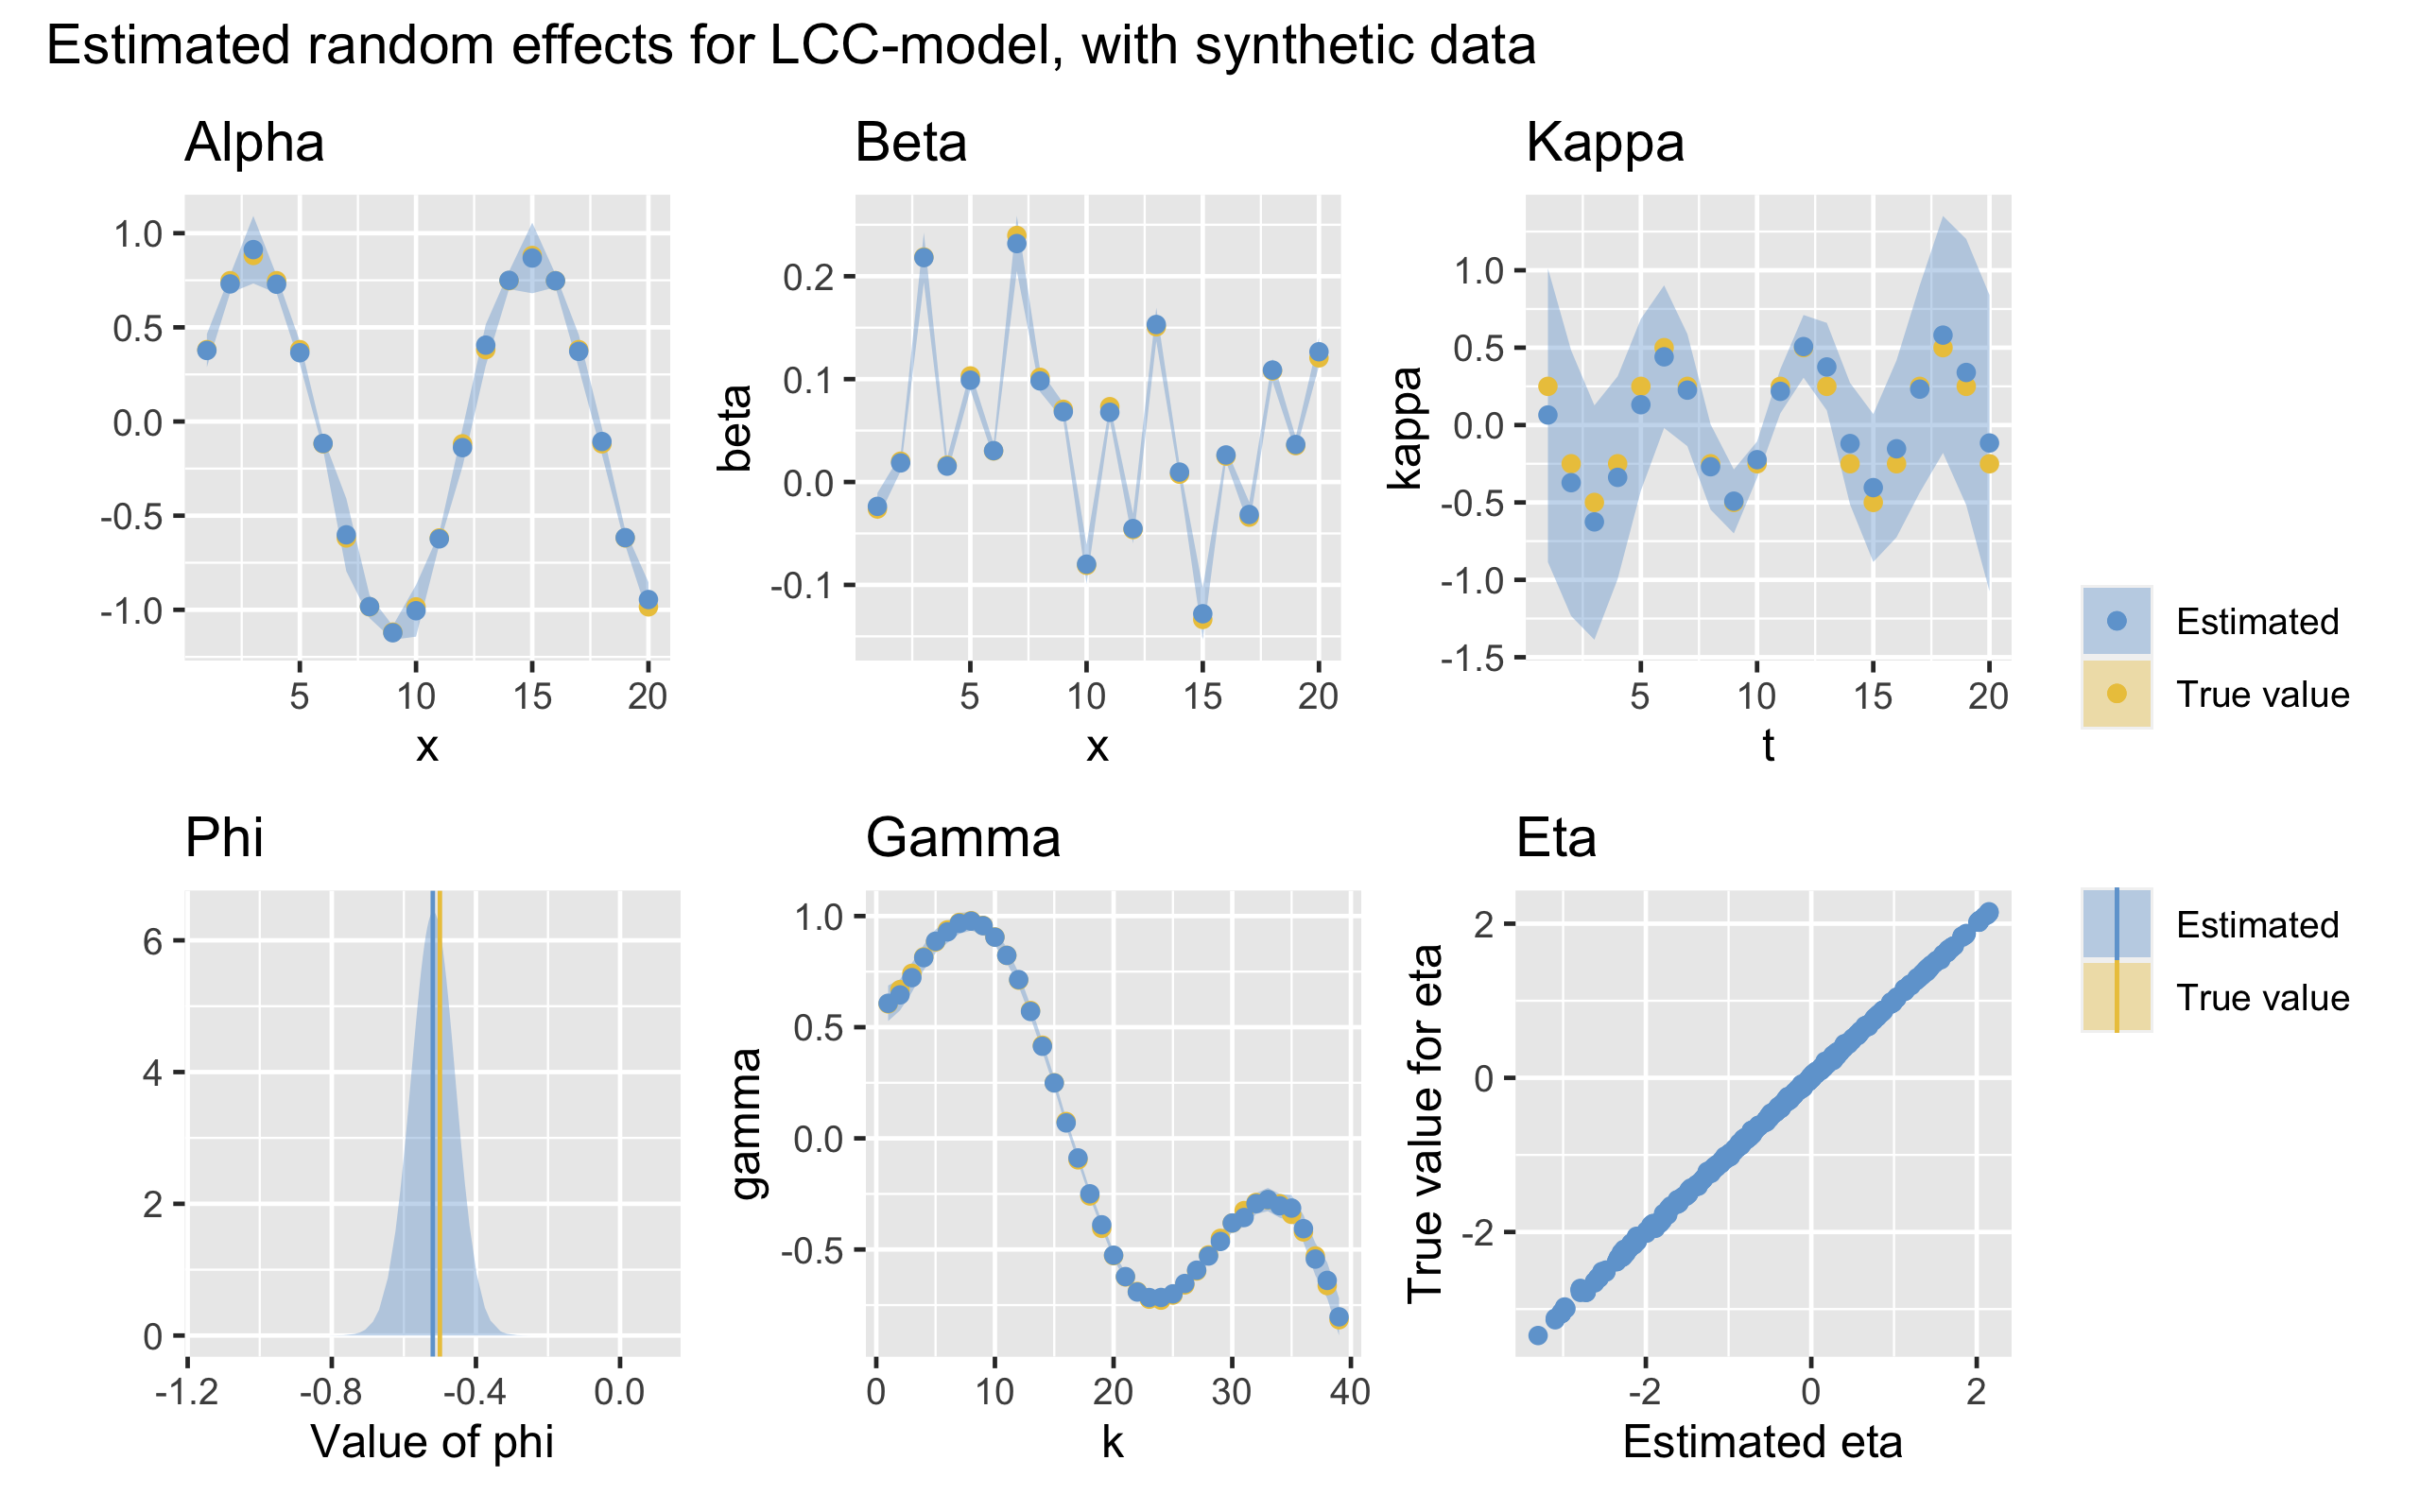
\includegraphics[width=\textwidth]{synthetic-data/Figures/effects-LCC-synthetic-3-1.png}
        \caption{The estimated random effects $\alpha_x$, $\beta_x$, $\phi$, $\kappa_t$ and $\gamma_k$, and the estimated predictor $\eta_{x,t}$}
        \label{fig:conf31-top}
    \end{subfigure}
    
    \begin{subfigure}[b]{0.6\textwidth}
        \centering
        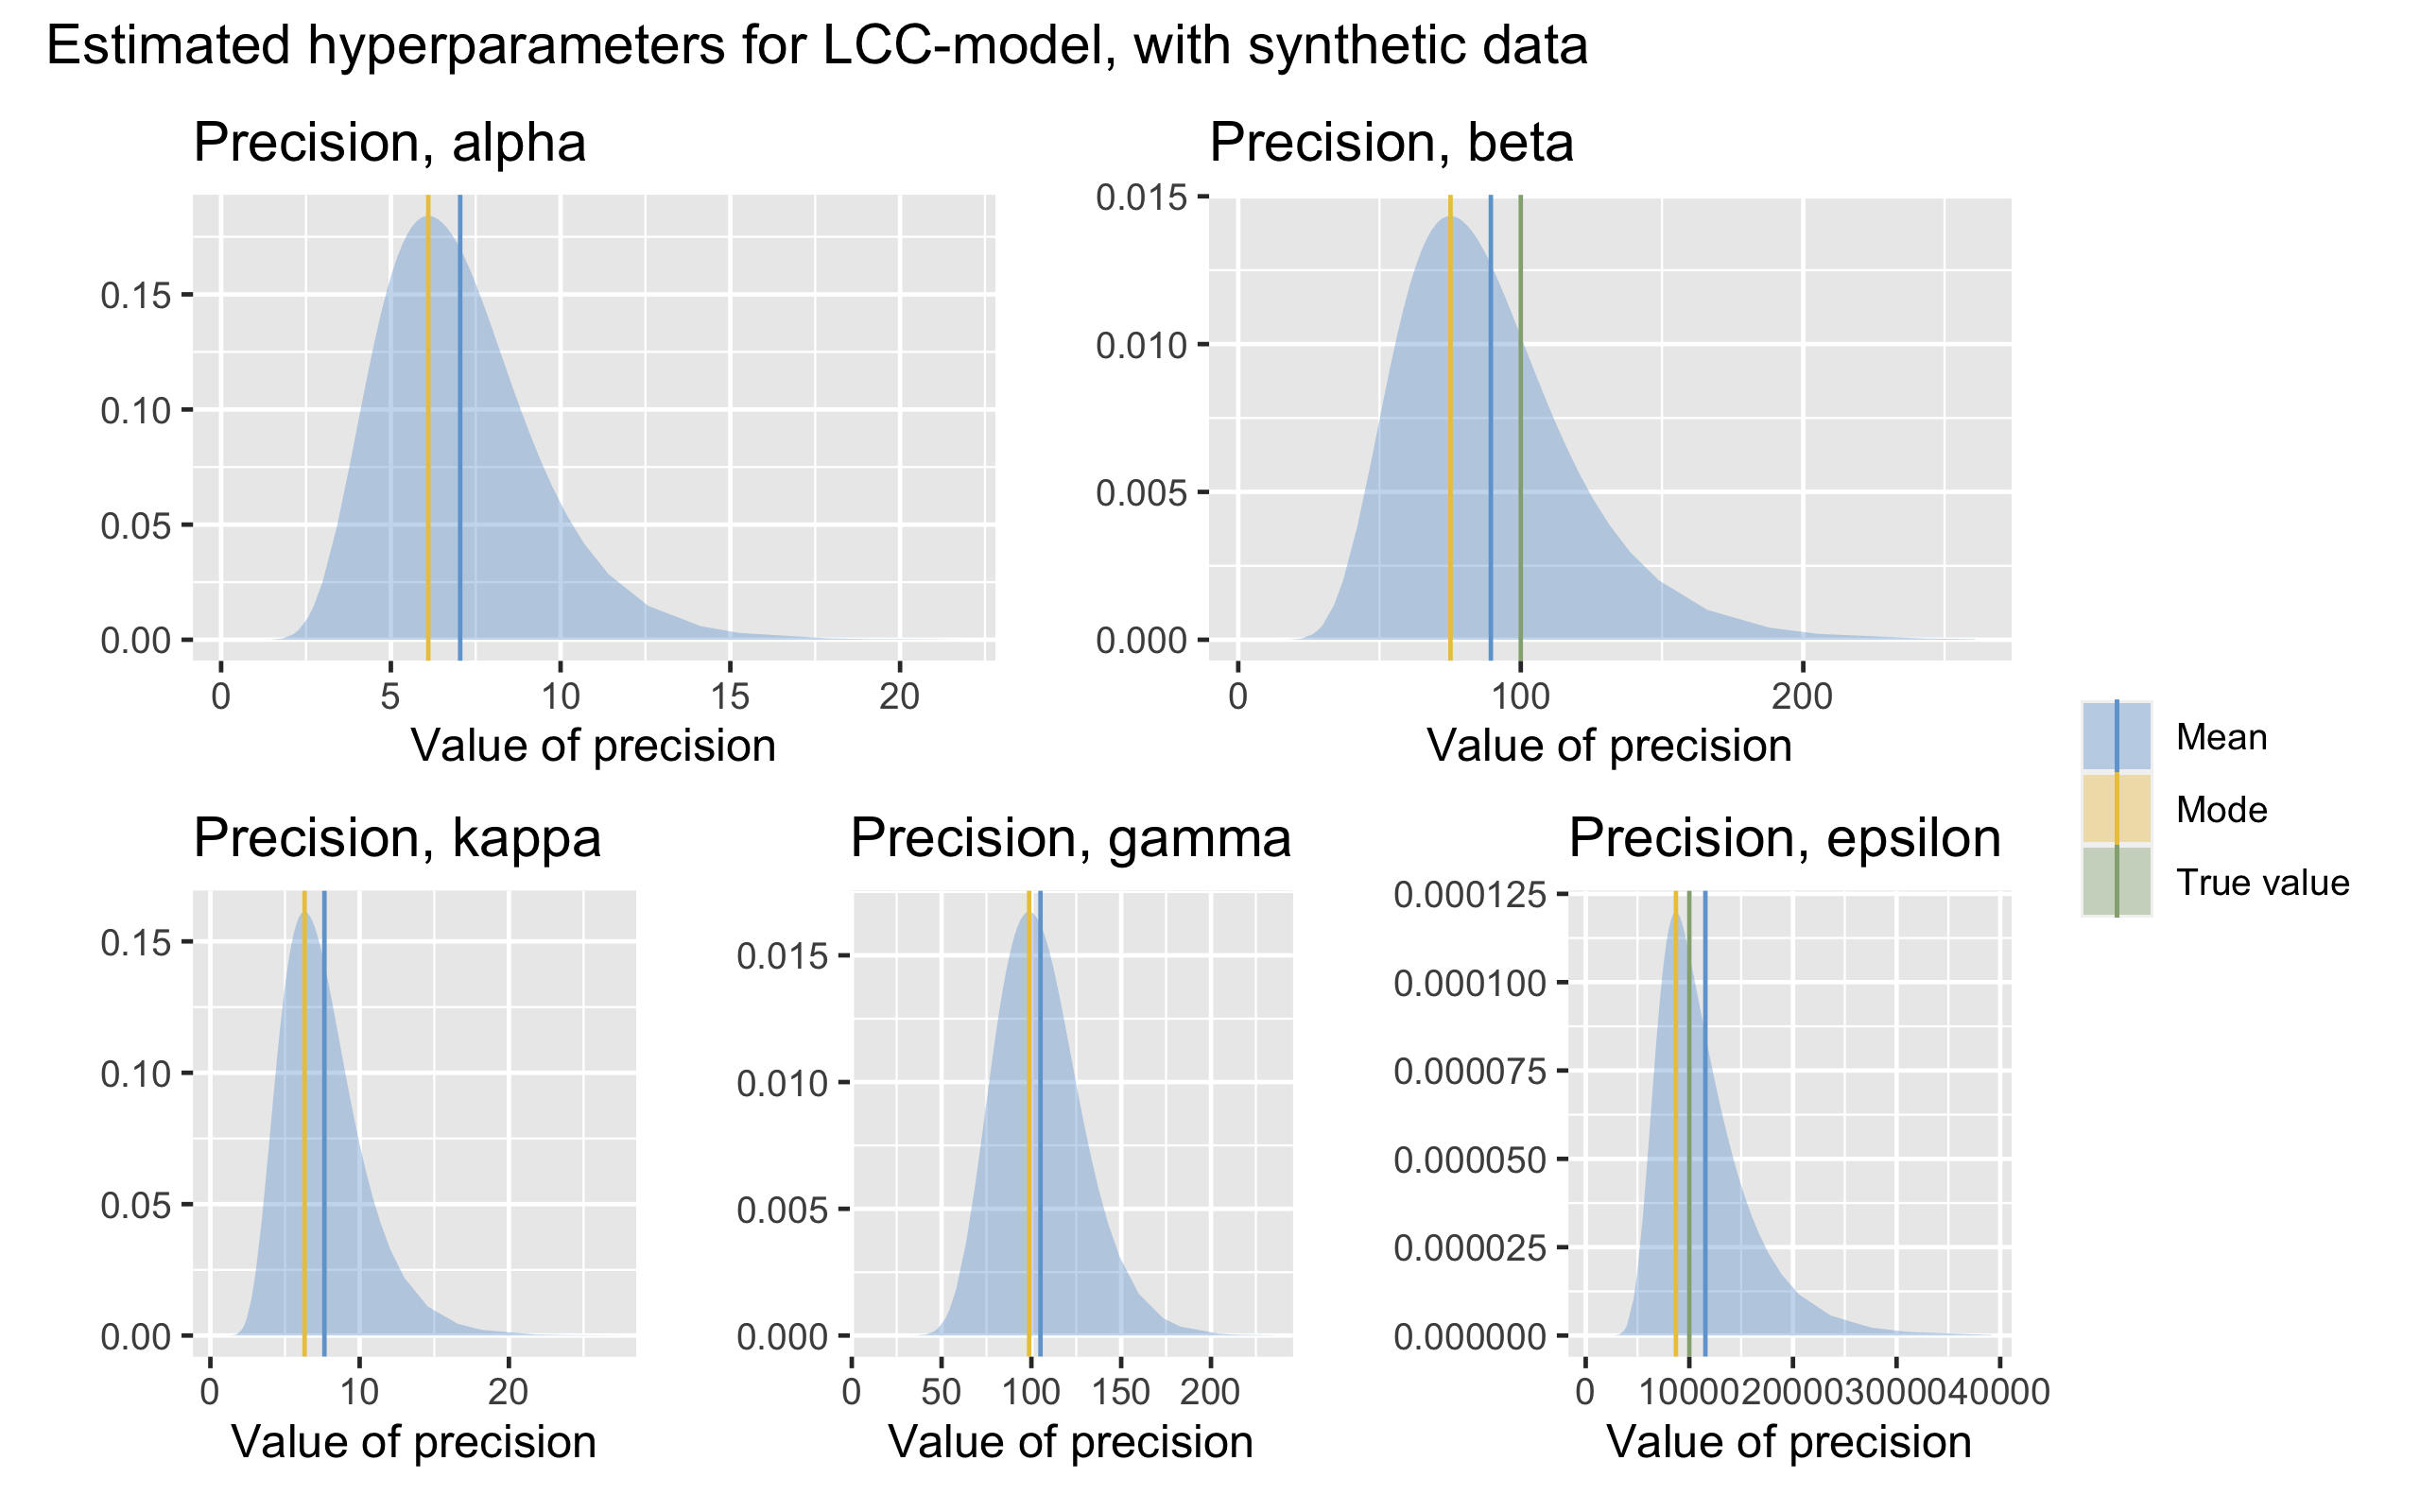
\includegraphics[width=\textwidth]{synthetic-data/Figures/hyperparameters-LCC-synthetic-3-1.png}
        \caption{The estimated precisions $\tau_\alpha$, $\tau_\beta$, $\tau_\kappa$, $\tau_\gamma$ and $\tau_\epsilon$.}
        \label{fig:conf31-bottom}
    \end{subfigure}
    \caption{Results from running \inlabru with the configuration of random effects given in Expression \ref{eq:conf31}. The plot layout is similar to that of Figure \ref{fig:firstRun}.}
    \label{fig:conf31}
\end{figure}

Figure \ref{fig:conf31} displays the results from running \inlabru when the random effects were simulated as
\begin{equation}
    \begin{aligned}
        &\alpha_x = \cos(\frac{x-3}{6}\pi)\\
        &\beta_x = \Normal(0,0.1^2)\\
        &\phi = -0.5\\
        &\kappa_t = \frac{1}{2}\cos(\frac{t\cdot \pi}{3})\\
        &\gammax = -\frac{1}{2}\left( 0.1k + \cos(\frac{k-2}{4})\right)\\
        &\tau_{\epsilon} = 1/0.01^2.
    \end{aligned}
    \label{eq:conf31}
\end{equation}
for $x\in[1,20]$, $t \in [1,20]$ and $k \in [1,39]$, where $\alpha_x$, $\beta_x$, $\kappa_t$ and $\gamma_k$ are adjusted to the constraints in Expression \ref{eq:LCconstraintsFinal}. 

\begin{figure}[h!]
    \centering
    \begin{subfigure}[b]{0.85\textwidth}
        \centering
        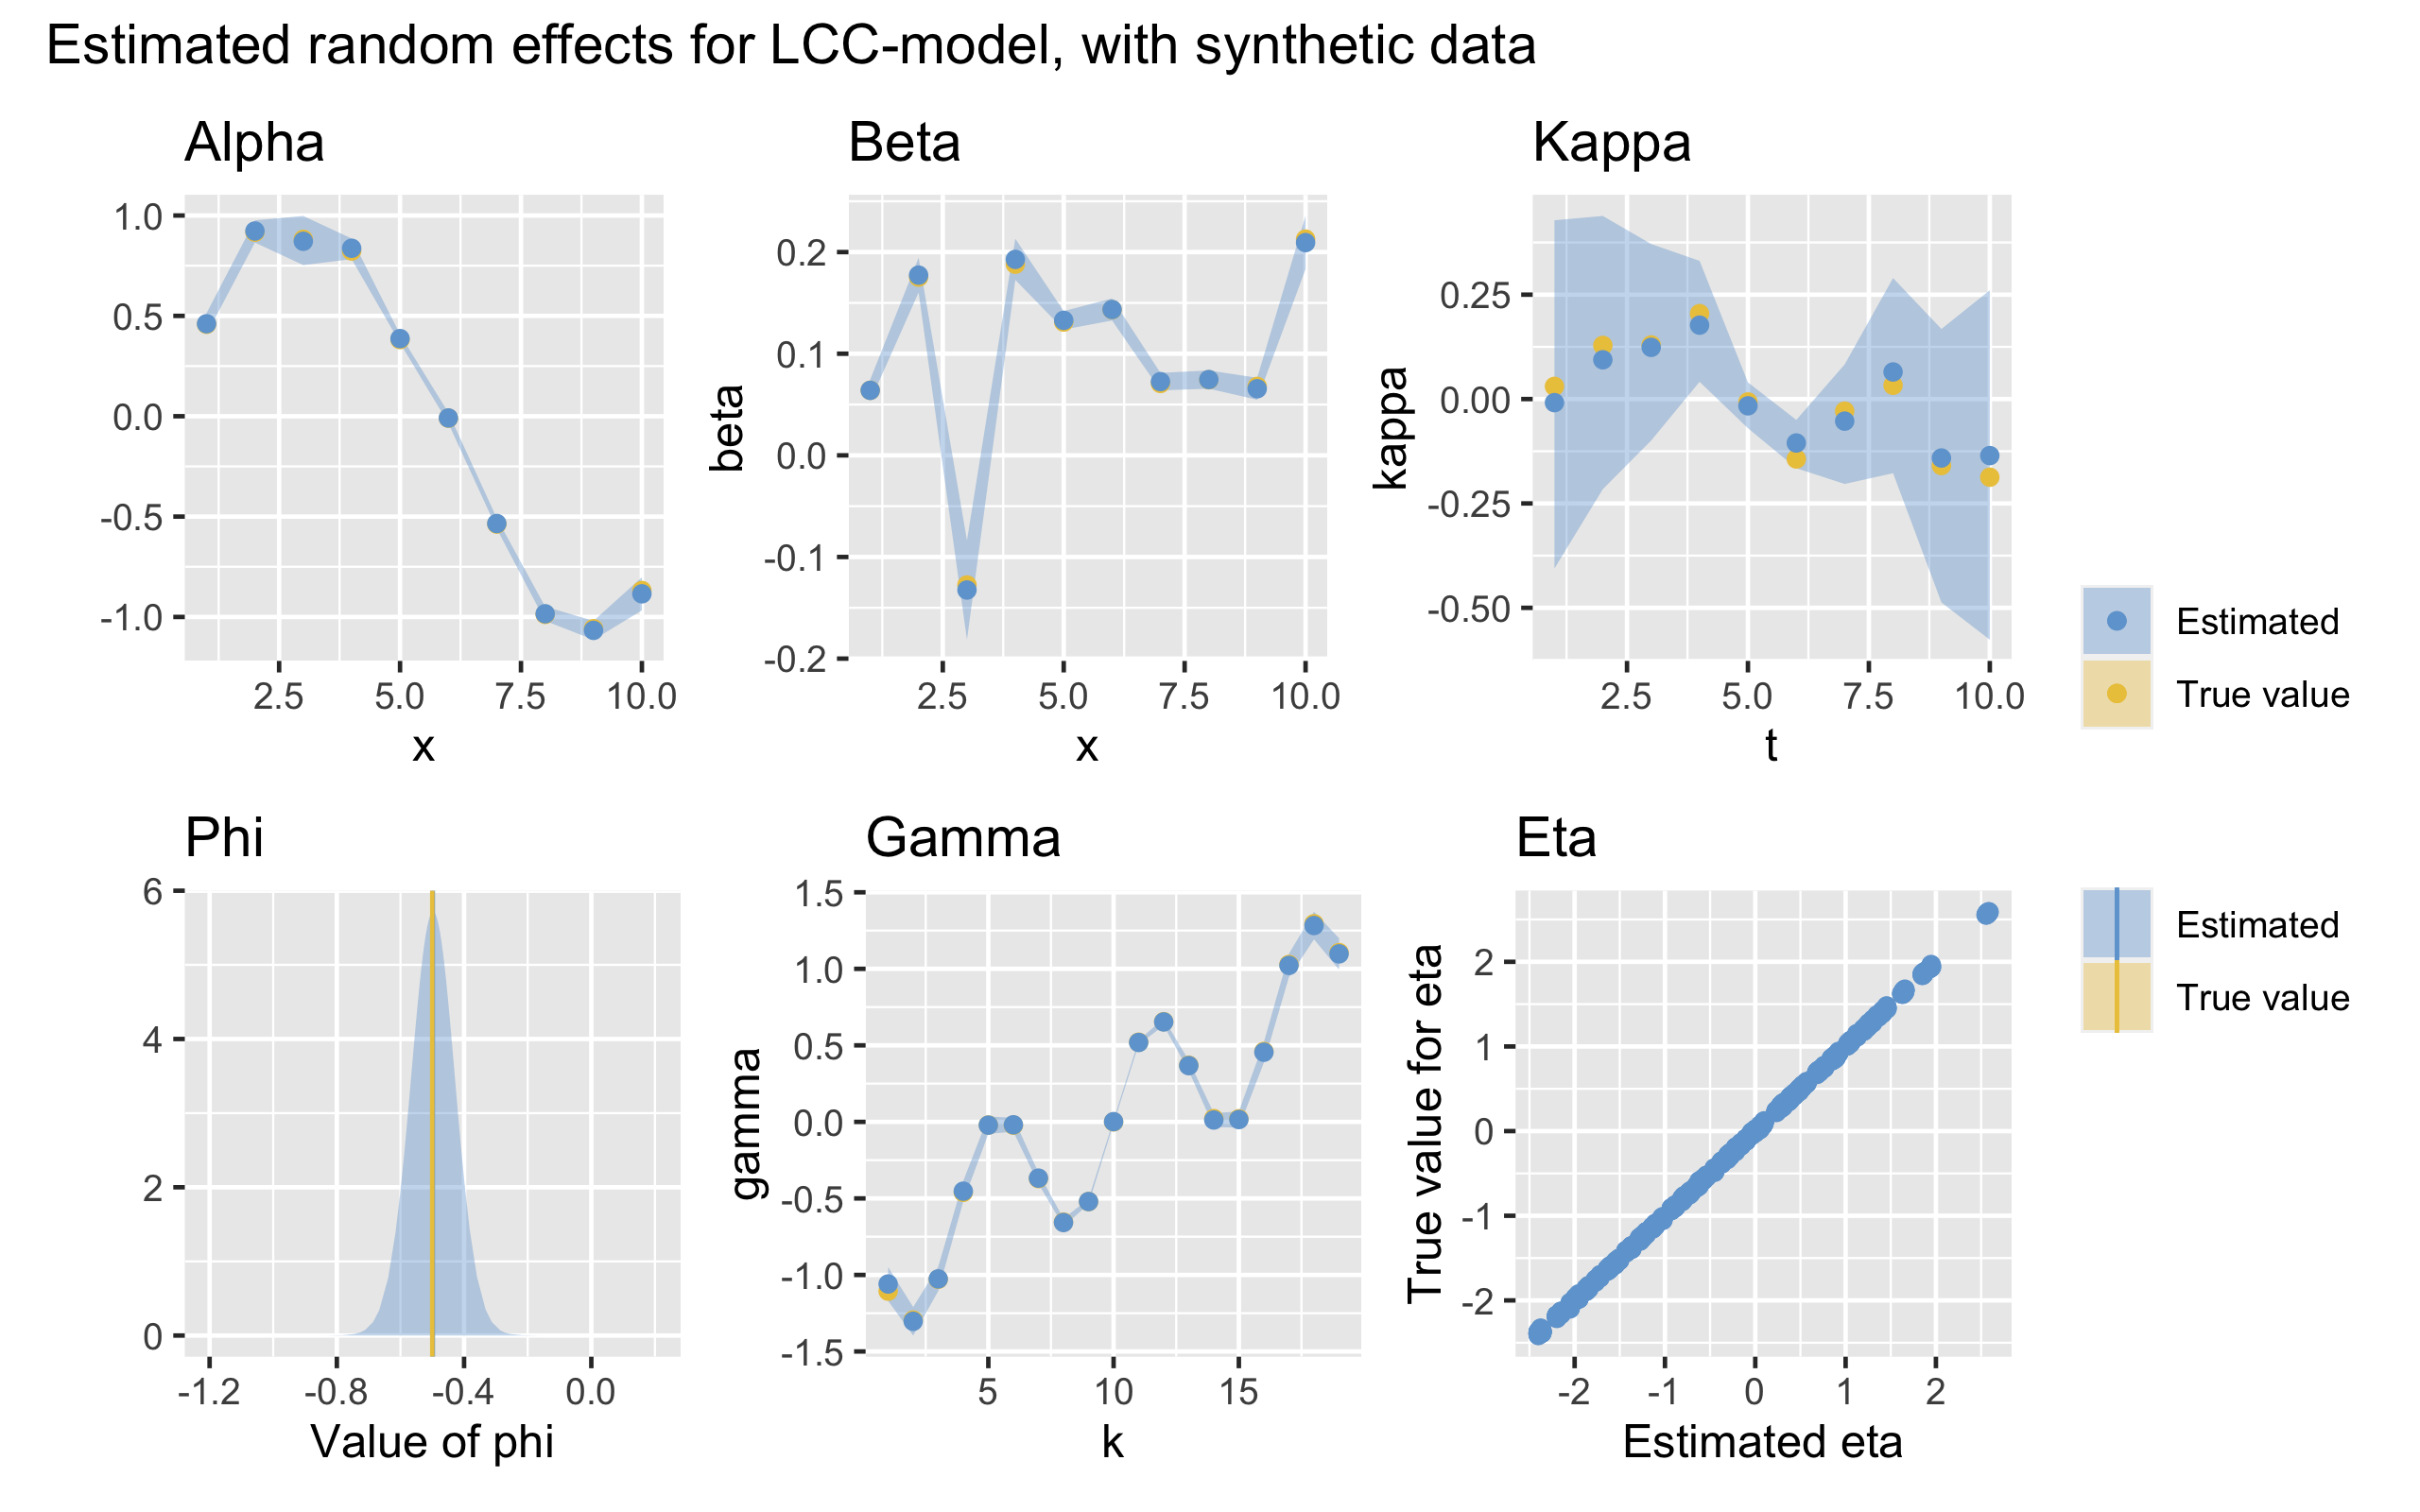
\includegraphics[width=\textwidth]{synthetic-data/Figures/effects-LCC-synthetic-3-2.png}
        \caption{The estimated random effects and the estimated $\eta_{x,t}$.}
        \label{fig:conf32-top}
    \end{subfigure}
    
    \begin{subfigure}[b]{0.6\textwidth}
        \centering
        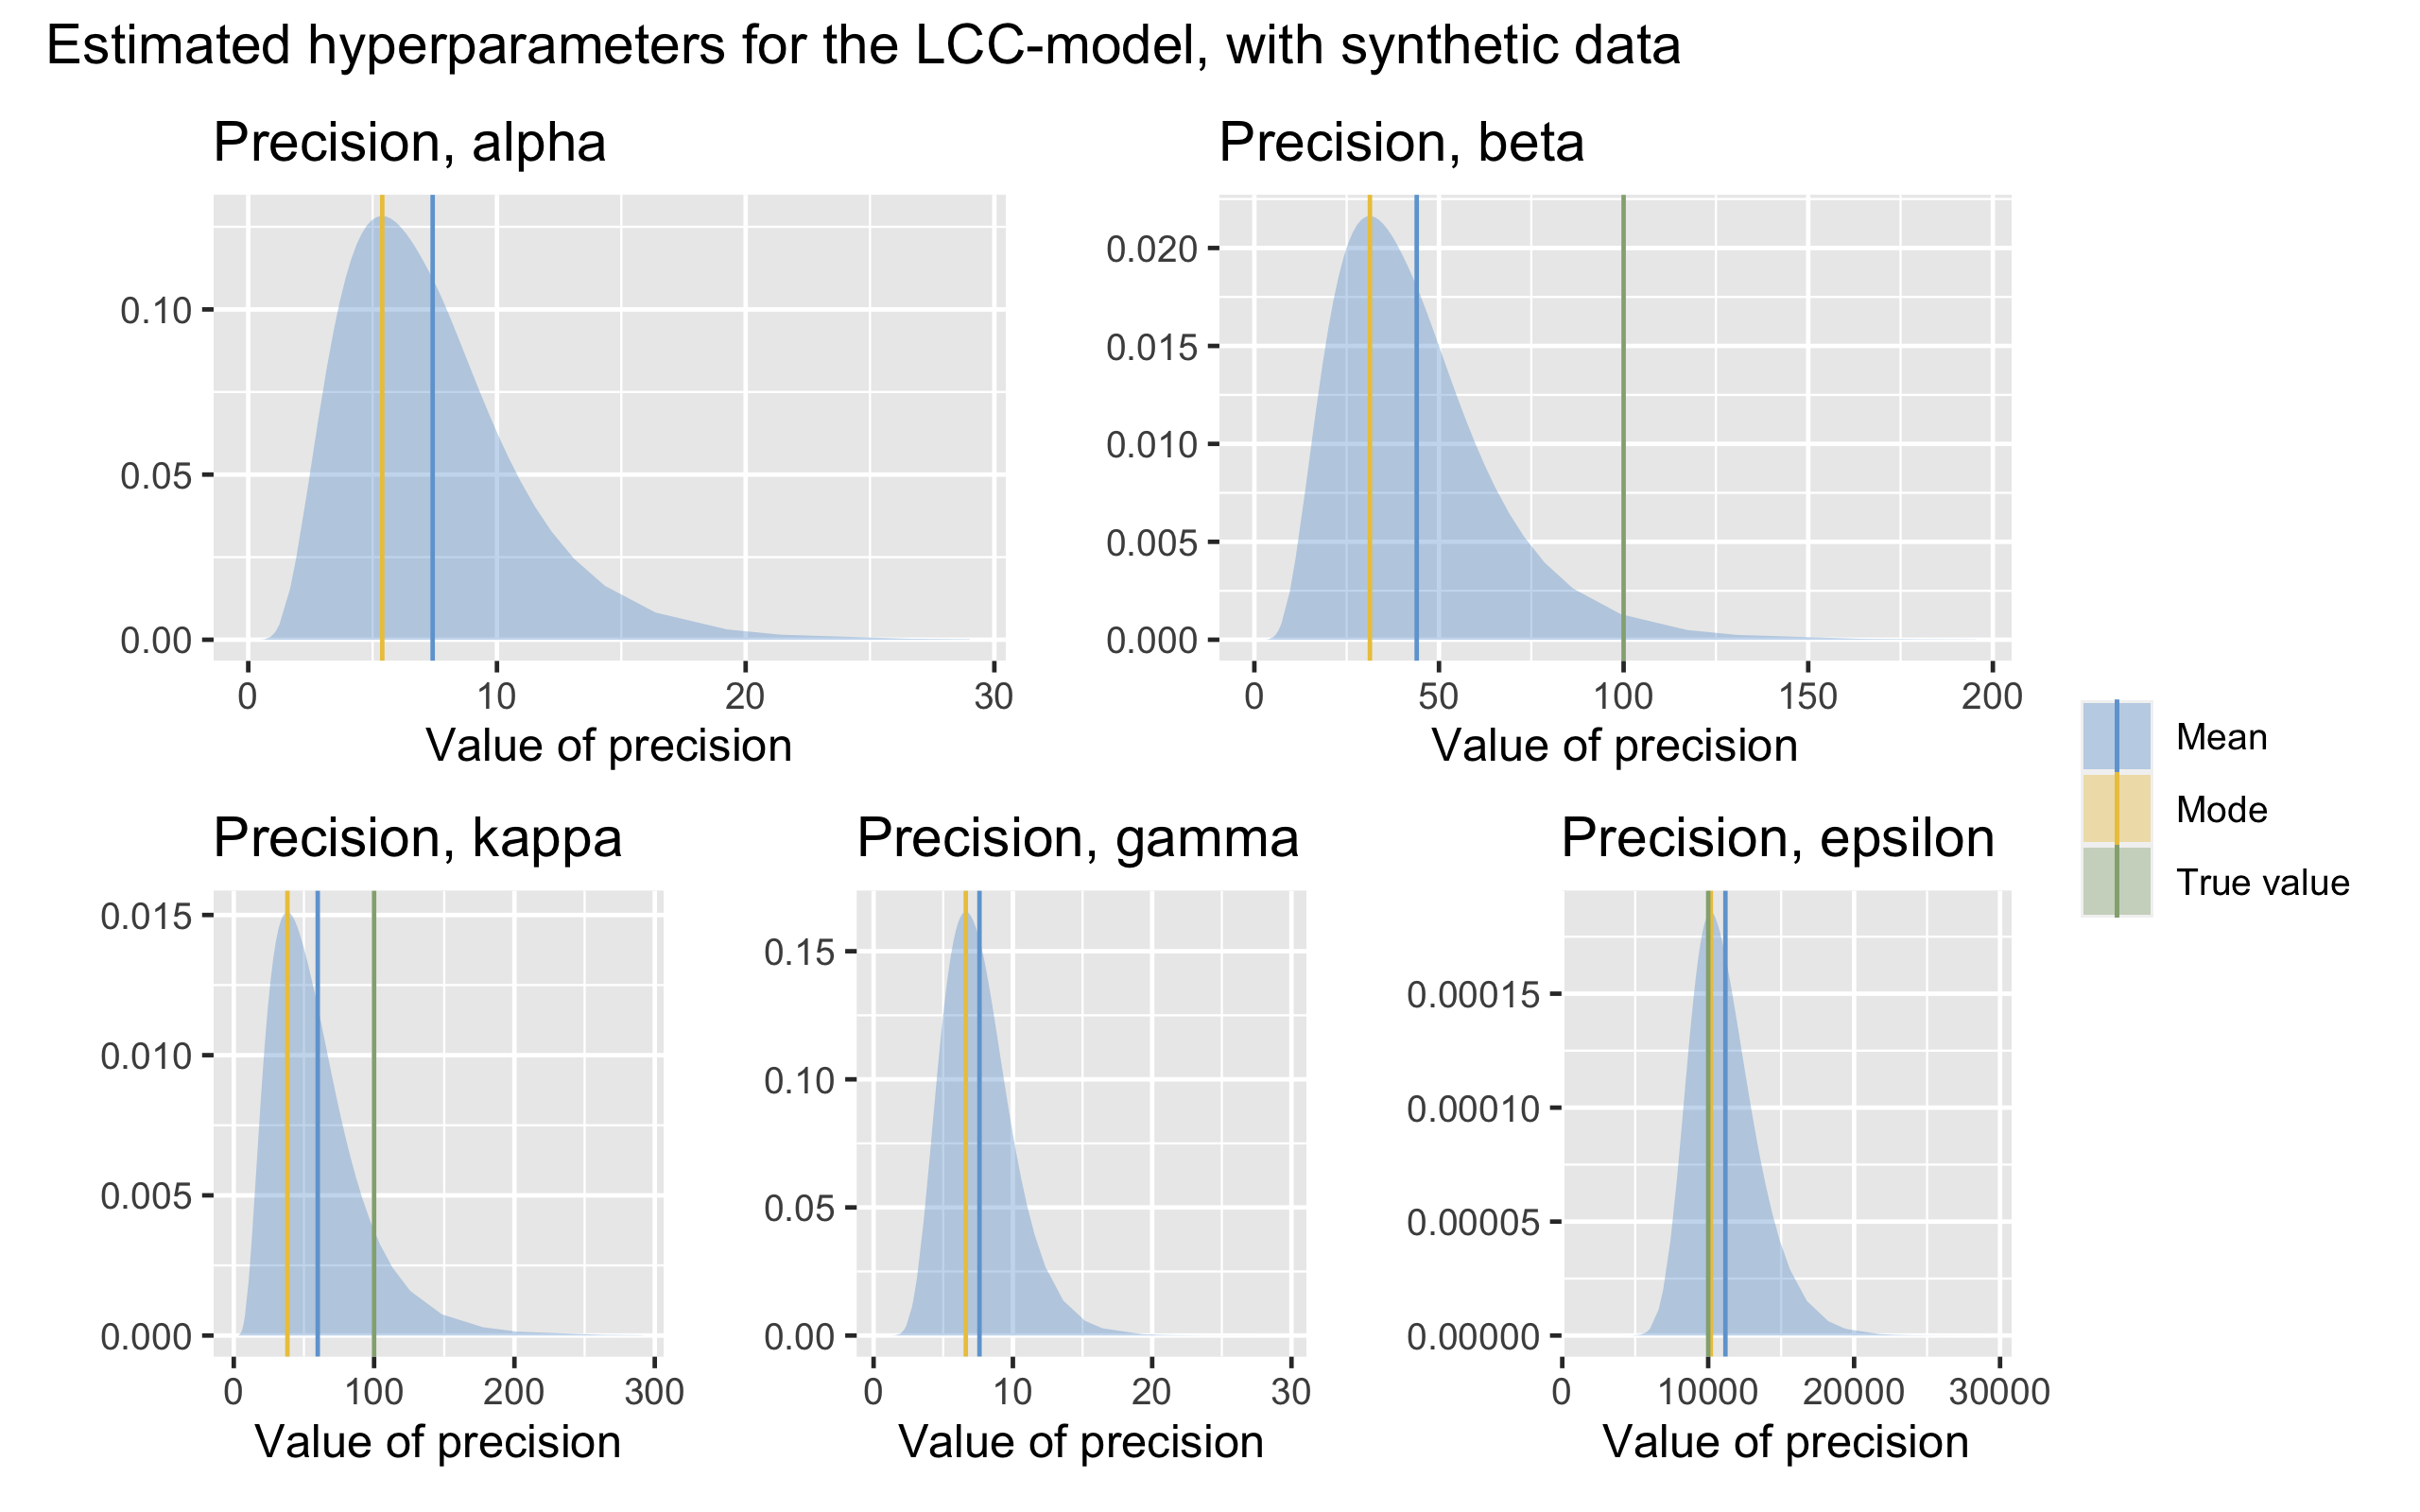
\includegraphics[width=\textwidth]{synthetic-data/Figures/hyperparameters-LCC-synthetic-3-2.png}
        \caption{The estimated precisions $\tau_\alpha$, $\tau_\beta$, $\tau_\kappa$, $\tau_\gamma$ and $\tau_\epsilon$. Since the true value of $\kappa_t$ from Configuration \ref{eq:conf32} is modelled as a random walk with the explicit precision $\tau_\kappa$, we include this true value of $\tau_\kappa$ as well as the true values for $\tau_\beta$ and $\tau_\epsilon$. }
        \label{fig:conf32-bottom}
    \end{subfigure}
    \caption{Results from running \inlabru with the configuration of random effects given in Expression \ref{eq:conf32}. The plot layout is similar to that of Figure \ref{fig:firstRun}.}
    \label{fig:conf32}
\end{figure}
Figure \ref{fig:conf32} displays the results from running \inlabru when the random effects are simulated as
\begin{equation}
    \begin{aligned}
        &\alpha_x = \cos(\frac{x-3}{6}\pi) + \epsilon_{x}, \quad \epsilon_{x} \sim \Normal(0,0.05^2)\\
        &\beta_x = \Normal(0,0.1^2)\\
        &\phi = -0.5\\
        &\kappa_t = RW1(0,0.1^2)\\
        &\gammax = \frac{1}{2}\left( 0.2k + \sin(k)\right)\\
        &\tau_{\epsilon} = 1/0.01^2.
    \end{aligned}
    \label{eq:conf32}
\end{equation}
for $x\in[1,10]$, $t \in [1,10]$ and $k \in [1,19]$, where $\alpha_x$, $\beta_x$, $\kappa_t$ and $\gamma_k$ are adjusted to the constraints in Expression \ref{eq:LCconstraintsFinal}. 

\begin{figure}[h!]
    \centering
    \begin{subfigure}[b]{0.85\textwidth}
        \centering
        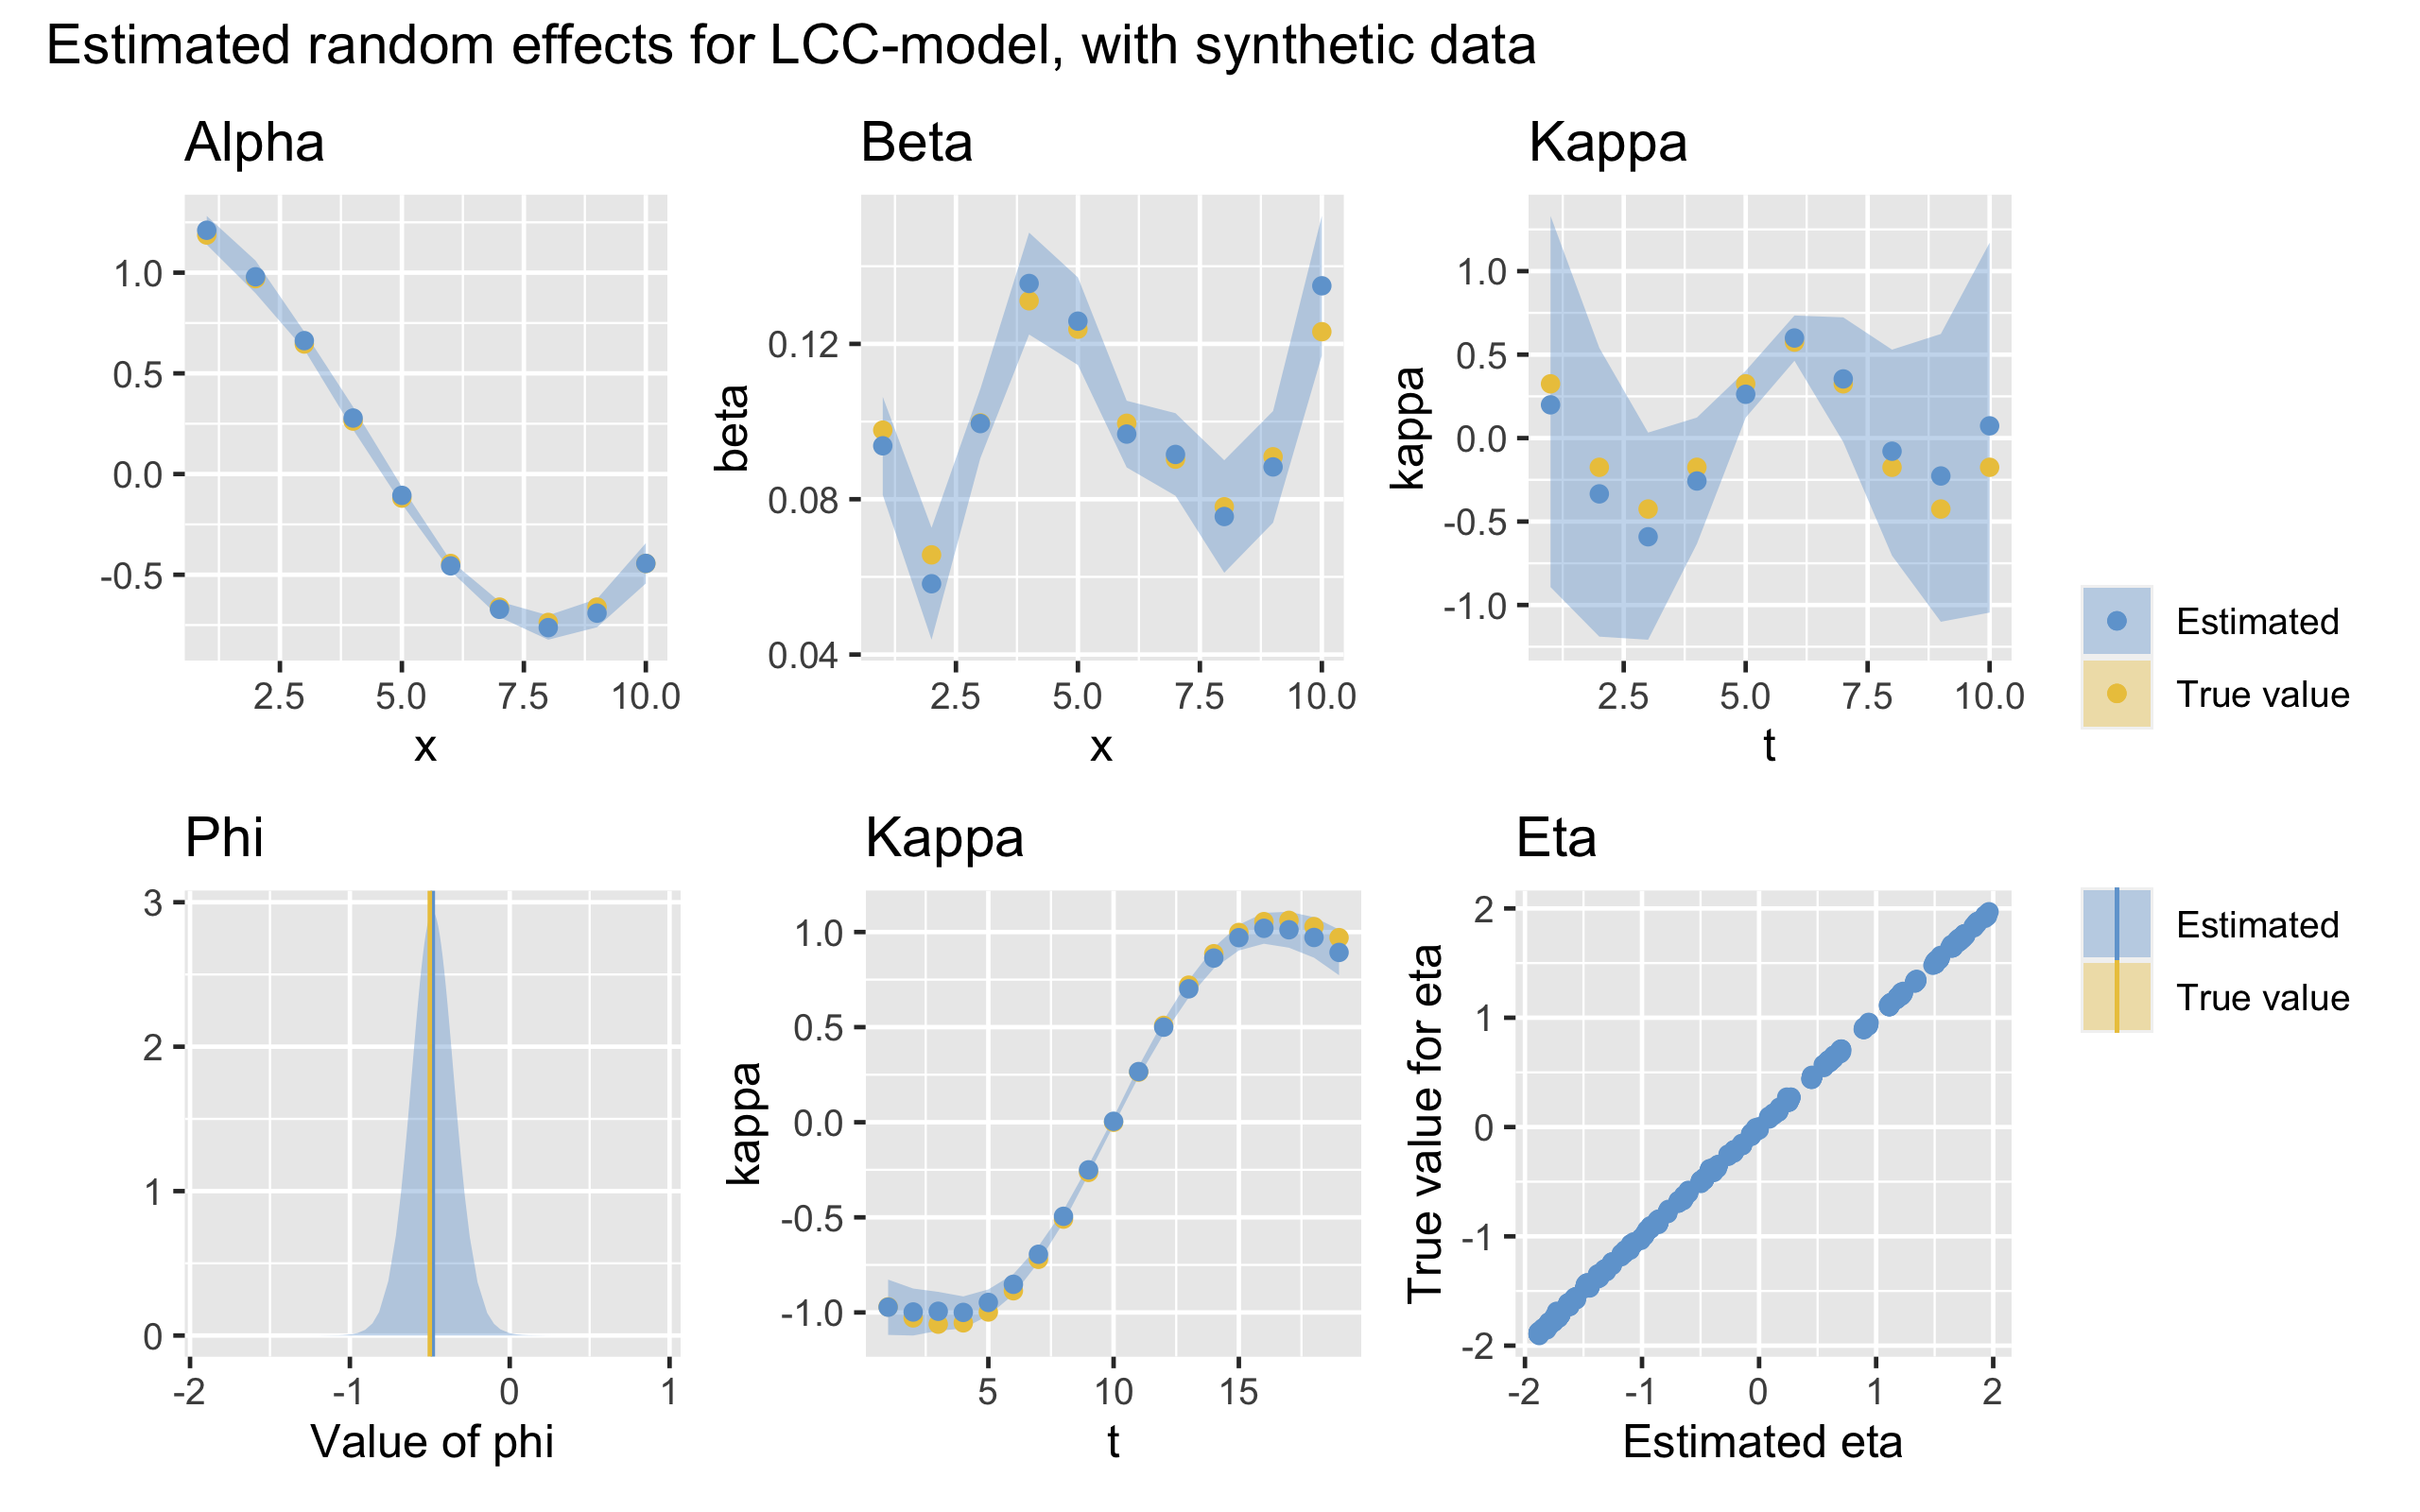
\includegraphics[width=\textwidth]{synthetic-data/Figures/effects-LCC-synthetic-3-3.png}
        \caption{The estimated random effects and the estimated $\eta_{x,t}$.}
        \label{fig:conf33-top}
    \end{subfigure}
    
    \begin{subfigure}[b]{0.6\textwidth}
        \centering
        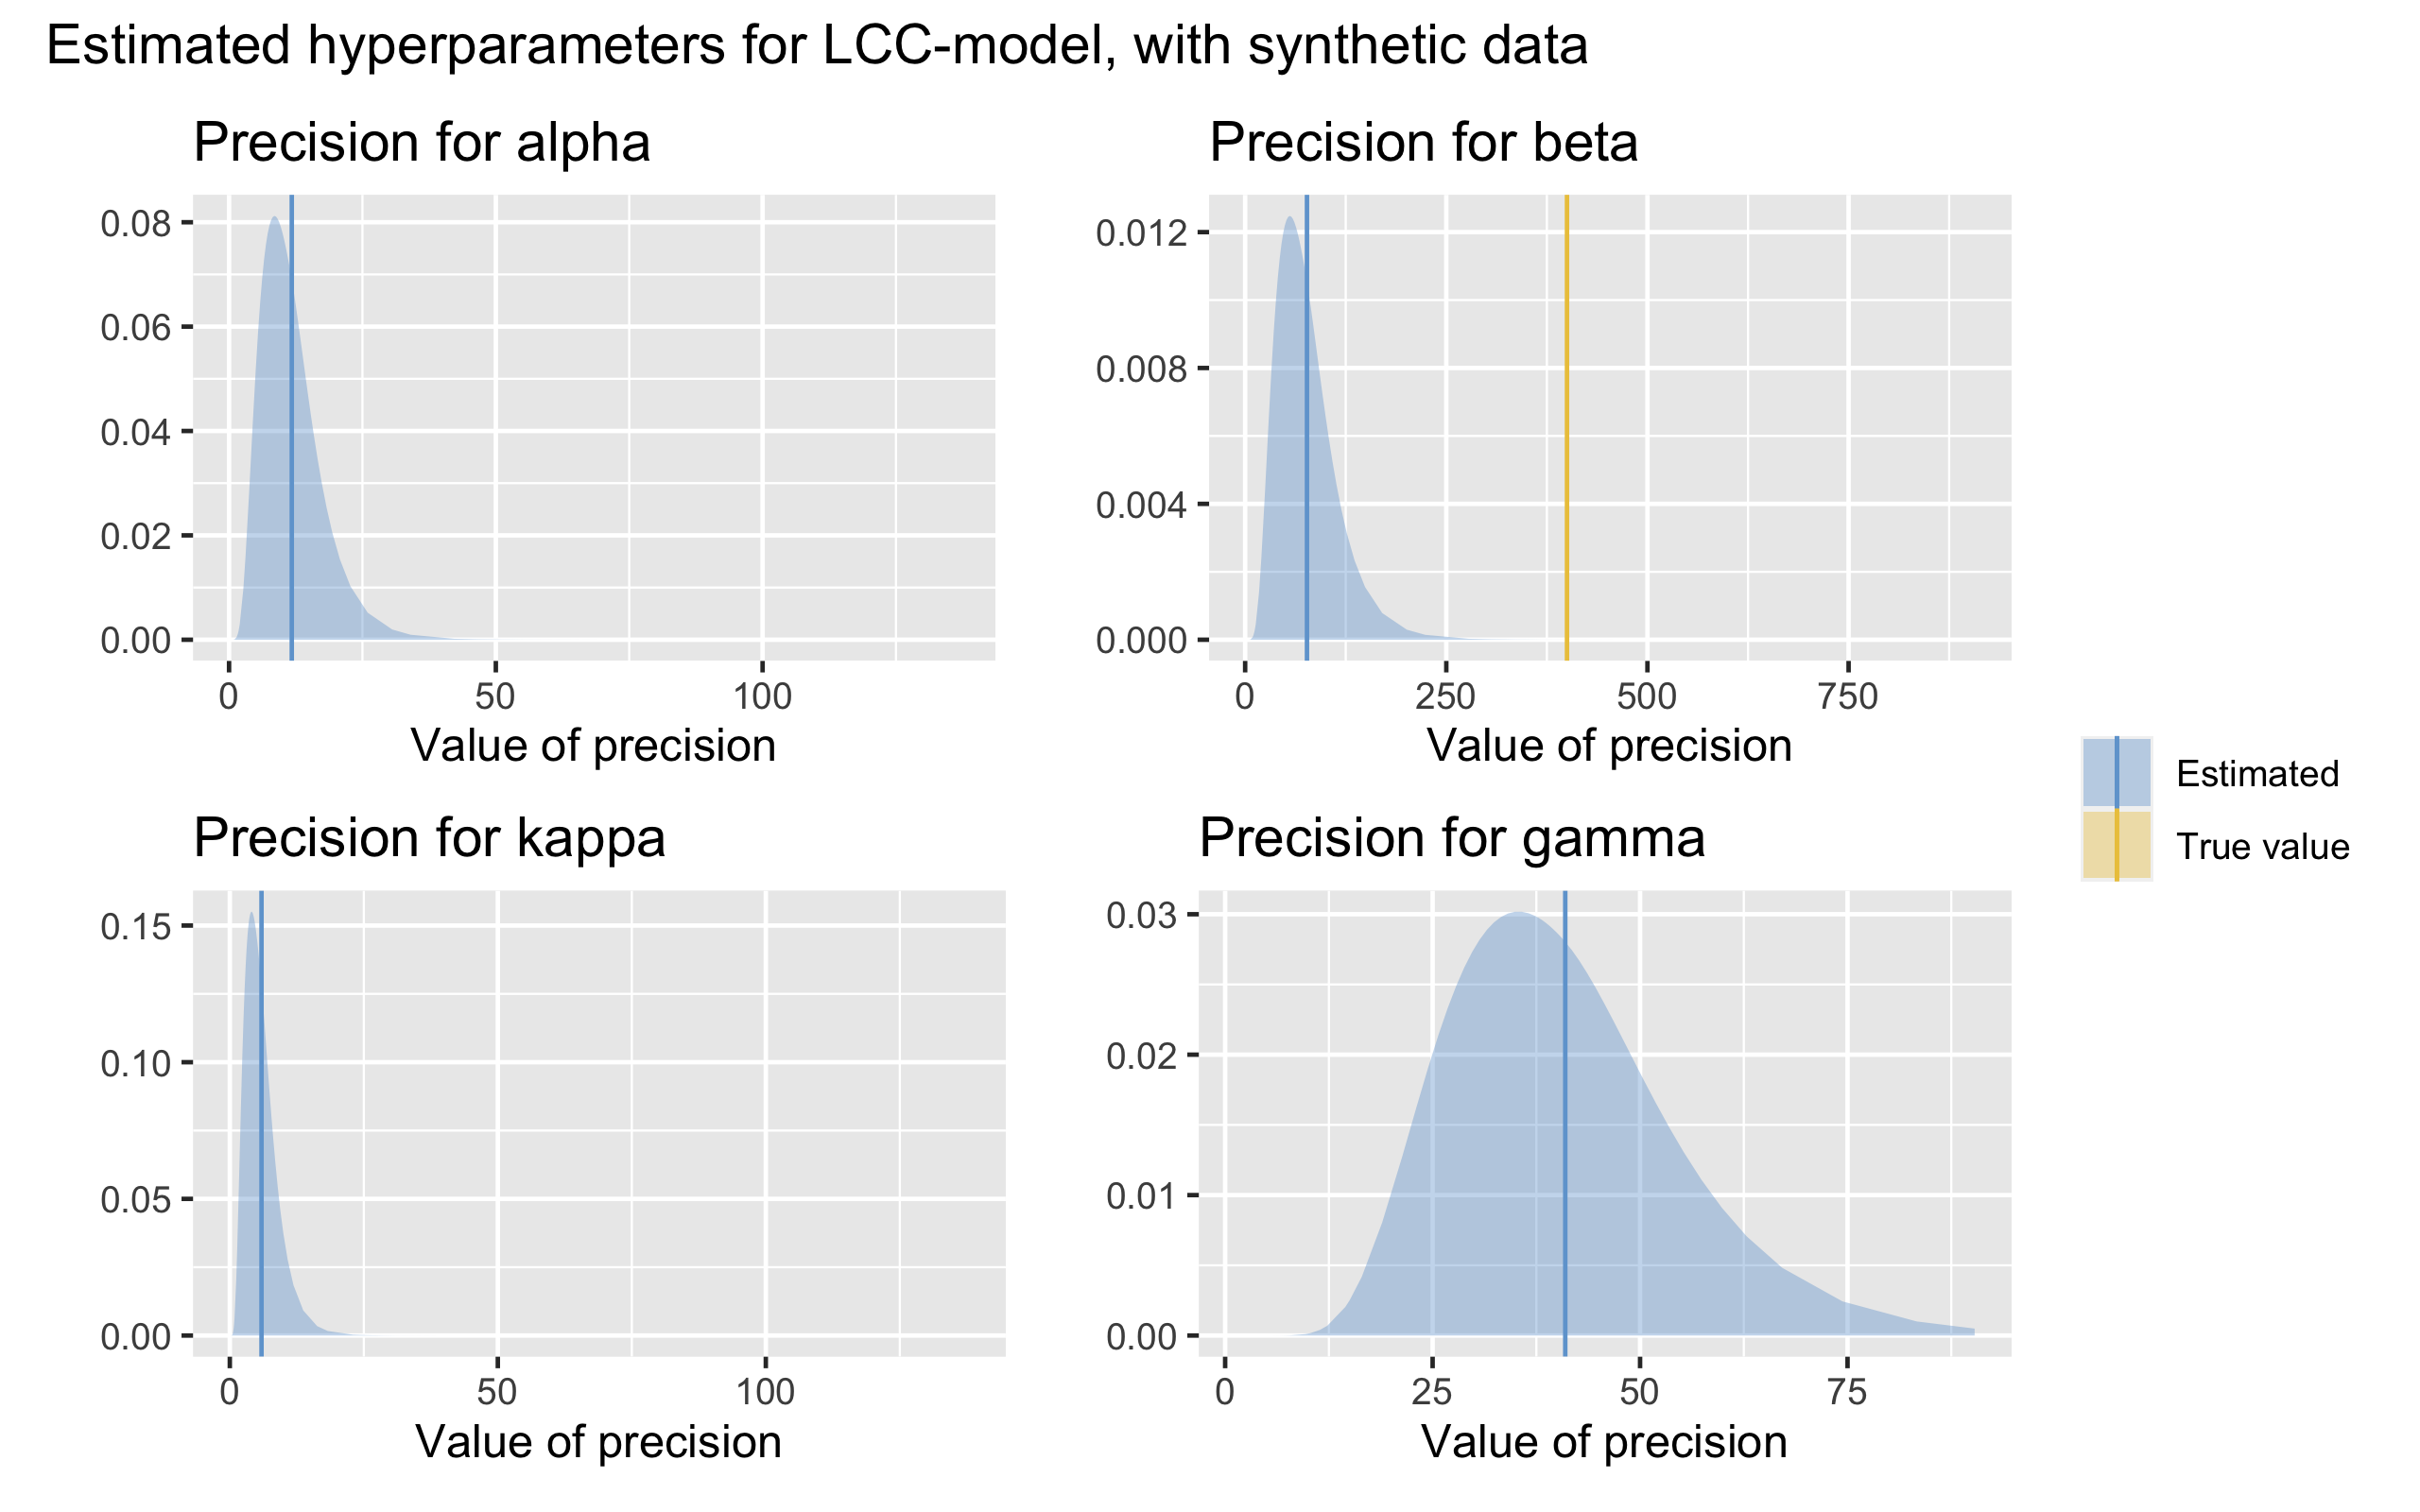
\includegraphics[width=\textwidth]{synthetic-data/Figures/hyperparameters-LCC-synthetic-3-3.png}
        \caption{The estimated precisions $\tau_\alpha$, $\tau_\beta$ and $\tau_\kappa$, $\tau_\gamma$ and $\tau_\epsilon$.}
        \label{fig:conf33-bottom}
    \end{subfigure}
    \caption{Results from running \inlabru with the configuration of random effects given in Expression \ref{eq:conf33}. The plot layout is similar to that of Figure \ref{fig:firstRun}.}
    \label{fig:conf33}
\end{figure}
Figure \ref{fig:conf33} displays the results from running \inlabru when the random effects are simulated as
\begin{equation}
    \begin{aligned}
        &\alpha_x = \cos(\frac{x}{8}\pi)\\
        &\beta_x = \Normal(0,0.05^2)\\
        &\phi = -0.5\\
        &\kappa_t = \frac{1}{2}\cos(\frac{t\pi}{3})\\
        &\gammax = \frac{1}{2}\left( 0.2k + \sin(k/3)\right)\\
        &\tau_{\epsilon} = 1/0.01^2.
    \end{aligned}
    \label{eq:conf33}
\end{equation}
for $x\in[1,10]$, $t \in [1,10]$ and $k \in [1,19]$, where $\alpha_x$, $\beta_x$, $\kappa_t$ and $\gamma_k$ are adjusted to the constraints in Expression \ref{eq:LCconstraintsFinal}. From Figures \ref{fig:conf31-top}, \ref{fig:conf32-top} and \ref{fig:conf33-top} we observe that \inlabru is able to estimate the random effects and the predictor $\eta_{x,t}$ well for the LCC-model, when fitted to data produced from the configurations given in Expressions \ref{eq:conf31}, \ref{eq:conf32} and \ref{eq:conf33}. 

\newpar Figures \ref{fig:conf31-bottom}, \ref{fig:conf32-bottom} and \ref{fig:conf33-bottom}, display the estimated precisions $\tau_\alpha$, $\tau_\beta$, $\tau_\kappa$, $\tau_\gamma$ and $\tau_\epsilon$. For all configurations, the estimated values of $\tau_\epsilon$ seem to align well with the true values. From Figure \ref{fig:conf31-bottom} and \ref{fig:conf32-bottom} we see that the estimated values of $\tau_\beta$, and $\tau_\kappa$ in the case of Figure \ref{fig:conf32-bottom}, are of the same order of magnitude as the true values from the corresponding configurations (in Expressions \ref{eq:conf31} and \ref{eq:conf32} respectively), although they are in general somewhat underestimated. From Figure \ref{fig:conf33-bottom} we observe that the underestimation of the value of $\tau_\beta$ compared to the true value of $\tau_\beta$ from Configuration \ref{eq:conf33} is more extreme. We also see, from Figure \ref{fig:conf33-top}, that the corresponding estimated values of $\beta_x$ have slightly wider confidence bounds than those of Figures \ref{fig:conf31-top} and \ref{fig:conf32-top}. However, this does not seem to affect the quality of the estimation of either $\eta_{x,t}$ or the remaining random effects, so we still say that the inference for the configuration in Expression \ref{eq:conf33} is successful. 

\newpar We test several other configurations of simulated effects, in addition to the three configurations described here, and we observe that most of them (excluding the types of configurations discussed in Section \ref{sec:IdentifiabilityKappa}) yield results similar to the examples displayed here. Considering this, we say that these results indicate that \inlabru is a suitable tool to perform Bayesian inference on LCC-models. 
